\section{Hệ bất phương trình bậc nhất hai ẩn}
\setcounter{dang}{0}
\subsection{Tóm tắt lý thuyết}
\subsubsection{Khái niệm hệ bất phương trình bậc nhất hai ẩn}
\begin{boxdn}
	\textbf{\textit{Hệ bất phương trình bậc nhất hai ẩn}} là hệ gồm hai hay nhiều bất phương trình bậc nhất hai ẩn $x$, $y$. Mỗi nghiệm chung của tất cả các bất phương trình đó được gọi là một nghiệm của hệ bất phương trình đã cho.\\
	Trên mặt phẳng toạ độ $Oxy$, tập hợp các điểm $(x_0;y_0)$ có tọa độ là nghiệm của hệ bất phương trình bậc nhất hai ẩn được gọi là \textbf{\textit{miền nghiệm}} của hệ bất phương trình đó.
\end{boxdn}
\subsubsection{Biểu diễn miền nghiệm của hệ bất phương trình bậc nhất hai ẩn}
\begin{boxdn}
	Để \textbf{\textit{biểu diễn miền nghiệm}} của hệ bất phương trình bậc nhất hai ẩn trên mặt phẳng toạ độ $Oxy$, ta thực hiện như sau:
	\begin{itemize}
	\item Trên cùng mặt phẳng tọa độ, biểu diễn miền nghiệm của mỗi bất phương trình của hệ.
	\item Phần giao của các miền nghiệm là miền nghiệm của hệ bất phương trình.
	\end{itemize}
\end{boxdn}
\begin{note}
	Miền mặt phẳng tọa độ bao gồm một đa giác lồi và phần nằm bên trong đa giác đó được gọi là một miền đa giác.
\end{note}
\subsubsection{Tìm giá trị lớn nhất và giá trị nhỏ nhất của biểu thức $\mathbf{F=ax+by}$ trên một miền đa giác}
Hệ bất phương trình giúp ta mô tả được nhiều bài toán thực tế để tìm ra cách giải quyết tối ưu. Chúng thường được đưa về bài toán tìm giá trị lớn nhất (GTLN) hoặc giá trị nhỏ nhất (GTNN) của biểu thức $F=ax+by$ trên một miền đa giác.\\
Người ta chứng minh được $F$ đạt giá trị lớn nhất hoặc nhỏ nhất tại một trong các đỉnh của đa giác.
\subsection{Các dạng toán}
\begin{dang}{Biểu diễn hình học của tập nghiệm}
	
\end{dang}

\viduminhhoa
\begin{vd}%[0D4B4]
	Biểu diễn hình học tập nghiệm của hệ bất phương trình bậc nhất hai ẩn sau
	$$\left\{\begin{aligned}
		x+y &> 1\\
		x-y &<2 \\
	\end{aligned}\right.$$
	\loigiai
	{\immini{
			Vẽ các đường thẳng
			\begin{gather*}
				d_1: x+y=1,
				d_2: x-y=2.
			\end{gather*}
			Vì điểm $M(0,2)$ có tọa độ thỏa mãn các bất phương trình trong hệ nên ta tô đậm các nửa mặt phẳng bờ $d_1,d_2$ không chứa $M$. 
			
			Miền không bị tô đậm trong hình vẽ và không chứa các tia giới hạn miền là miền nghiệm của hệ đã cho.
		}{
			\begin{tikzpicture}[line cap=round, line join=round, font=\footnotesize, >=stealth, scale=1]
				\tikzset{label style/.style={font=\footnotesize}}
				\draw[color=white,fill=black!10] (-2,-2) rectangle (4,3);
				\draw[fill=white,color=white] (-2,3) -- (1.5,-.5) -- (4,2) -- (4,3) -- cycle;
				\draw[->] (0,-2) -- (0,3) node[left]{\scriptsize $y$};
				\draw[->] (-2,0) -- (4,0) node[above]{\scriptsize $x$};
				\draw (0.15,0.1) node[below left]{\scriptsize $O$};
				\draw (-2,3) -- (3,-2) node[right]{\scriptsize $d_1$};
				\draw (0,-2) -- (4,2) node[right]{\scriptsize $d_2$};
				\draw[dashed] (0,-0.5)node[left]{\scriptsize $-\dfrac{1}{2}$} -- (1.5,-.5) node[right]{\scriptsize $I$} -- (1.5,0) node[above]{\scriptsize $\dfrac{3}{2}$};
				\draw (0,2) node[right]{\scriptsize $M$} (0,2) node[left]{\scriptsize $2$} (-0.05,2) -- (0.05,2);
			\end{tikzpicture}
		}
	}
\end{vd}
\begin{vd}%[0D4B4]
	Biểu diễn hình học tập nghiệm của hệ bất phương trình bậc nhất hai ẩn sau
	$$\left\{\begin{aligned}
		x+y &< 2\\
		x-y &>1 \\
		y &>-1
	\end{aligned}\right.$$
	\loigiai
	{\immini{
			Vẽ các đường thẳng
			\begin{gather*}
				d_1: x+y=2,\\
				d_2: x-y=1,\\
				d_3: y=-1.
			\end{gather*}
			Vì điểm $M\biggl(\dfrac{3}{2},0\biggr)$ có tọa độ thỏa mãn các bất phương trình trong hệ nên ta tô đậm các nửa mặt phẳng bờ $d_1,d_2,d_3$ không chứa $M$. Miền không bị tô đậm trong hình vẽ, không bao gồm các đoạn giới hạn miền là miền nghiệm của hệ đã cho.
		}{
			\begin{tikzpicture}[line cap=round, line join=round, font=\footnotesize, >=stealth, scale=1]
				\tikzset{label style/.style={font=\footnotesize}}
				\draw[color=white,fill=black!10] (-2,-2) rectangle (5,3);
				\path (-1,3) coordinate (A1);
				\path (4,-2) coordinate (B1);
				\path (-1,-2) coordinate (A2);
				\path (4,3) coordinate (B2);
				\path (-2,-1) coordinate (A3);
				\path (5,-1) coordinate (B3);
				\path (intersection of A1--B1 and A2--B2) coordinate (A);
				\path (intersection of A1--B1 and A3--B3) coordinate (B);
				\path (intersection of A2--B2 and A3--B3) coordinate (C);
				\draw[fill=white] (A) -- (B) -- (C) -- cycle;
				\draw[->] (0,-2) -- (0,3) node[right]{\scriptsize $y$};
				\draw[->] (-2,0) -- (5,0) node[above]{\scriptsize $x$};
				\draw (0,0) node[above left]{\scriptsize $O$};
				\draw (A1) -- (B1) node[right]{\scriptsize $d_1$} (A2) -- (B2)node[right]{\scriptsize $d_2$} (A3) -- (B3)node[right]{\scriptsize $d_3$};
				\draw[dashed] (B)node[below]{\scriptsize $B$} -- (B |- 0,0) node[above]{\scriptsize $3$}
				(A-| 0,0)node[left]{\scriptsize $\dfrac{3}{2}$} -- (A)node[above]{\scriptsize $A$} -- (A|- 0,0)node[below]{\scriptsize $\dfrac{3}{2}$};
				\draw (1.5,0)node[above right]{\scriptsize $M$} (C) node[below right]{\scriptsize $C$} (C) node[above left]{\scriptsize $-1$};
			\end{tikzpicture}
		}
	}
\end{vd}
\begin{vd}%[0D4B4]
	Biểu diễn hình học tập nghiệm của hệ bất phương trình bậc nhất hai ẩn sau
	$$\left\{\begin{aligned}
		2x+5y &> 2\\
		x-3y &\geq 1 \\
		x+y &<3
	\end{aligned}\right.$$
	\loigiai
	{\immini{
			Vẽ các đường thẳng
			\begin{gather*}
				d_1: 2x+5y=2,\\
				d_2: x-3y=1,\\
				d_3: x+y=3.
			\end{gather*}
			Vì điểm $M(2,0)$ có tọa độ thỏa mãn các bất phương trình trong hệ nên ta tô đậm các nửa mặt phẳng bờ $d_1,d_2,d_3$ không chứa $M$. 
			
			Miền không bị tô đậm trong hình vẽ có chứa đoạn $AC$ và không chứa các điểm $A,C$, không chứa các đoạn $AB,BC$ là miền nghiệm của hệ đã cho.
		}{
			\begin{tikzpicture}[line cap=round, line join=round, font=\footnotesize, >=stealth, scale=1]
				\tikzset{label style/.style={font=\footnotesize}}
				\draw[color=white,fill=black!10] (-1,-2) rectangle (6,3.2);
				\path (-1,0.8) coordinate (A1);
				\path (6,-2) coordinate (B1);
				\path (-1,-2/3) coordinate (A2);
				\path (6,5/3) coordinate (B2);
				\path (-0.2,3.2) coordinate (A3);
				\path (5,-2) coordinate (B3);
				\path (intersection of A1--B1 and A2--B2) coordinate (A);
				\path (intersection of A1--B1 and A3--B3) coordinate (B);
				\path (intersection of A2--B2 and A3--B3) coordinate (C);
				\draw[fill=white] (A) -- (B) -- (C) -- cycle;
				\draw[->] (0,-2) -- (0,3.2) node[right]{\scriptsize $y$};
				\draw[->] (-1,0) -- (6,0) node[above]{\scriptsize $x$};
				\draw (0.15,0.1) node[below left]{\scriptsize $O$};
				\draw (A1) -- (B1) node[right]{\scriptsize $d_1$} (A2) -- (B2)node[right]{\scriptsize $d_2$} (A3) -- (B3)node[right]{\scriptsize $d_3$};
				\draw[dashed] (B -| 0,0) node[left]{\scriptsize $-\dfrac{4}{3}$}--(B)node[below]{\scriptsize $B$} -- (B |- 0,0) node[above]{\scriptsize $\dfrac{13}{3}$}
				(C-| 0,0) node[left]{\scriptsize $\dfrac{1}{2}$} -- (C)node[above]{\scriptsize $C$} -- (C|- 0,0)node[below]{\scriptsize $\dfrac{5}{2}$};
				\draw (2,0)node[above]{\scriptsize $2$} (2,0.05)  -- (2,-0.05) node[below]{\scriptsize $M$} (A) node[below]{\scriptsize $A$} (A) node[above]{\scriptsize $1$};	
			\end{tikzpicture}
		}
	}
\end{vd}
\begin{vd}%[0D4B4]
	Biểu diễn hình học tập nghiệm của hệ bất phương trình bậc nhất hai ẩn sau
	$$\left\{\begin{aligned}
		2x+y &\geq 2\\
		x-2y &\leq 1 \\
		y &\leq 2\\
		x &\leq 3
	\end{aligned}\right.$$
	\loigiai
	{\immini{
			Vẽ các đường thẳng
			\begin{gather*}
				d_1: 2x+y=2,\\
				d_2: x-2y=1,\\
				d_3: y=2,
				d_4: x=3.
			\end{gather*}
			Vì điểm $M(2,1)$ có tọa độ thỏa mãn các bất phương trình trong hệ nên ta tô đậm các nửa mặt phẳng bờ $d_1,d_2,d_3,d_4$ không chứa $M$. Miền không bị tô đậm trong hình vẽ là miền nghiệm của hệ đã cho bao gồm các đoạn thẳng xác định miền.
		}{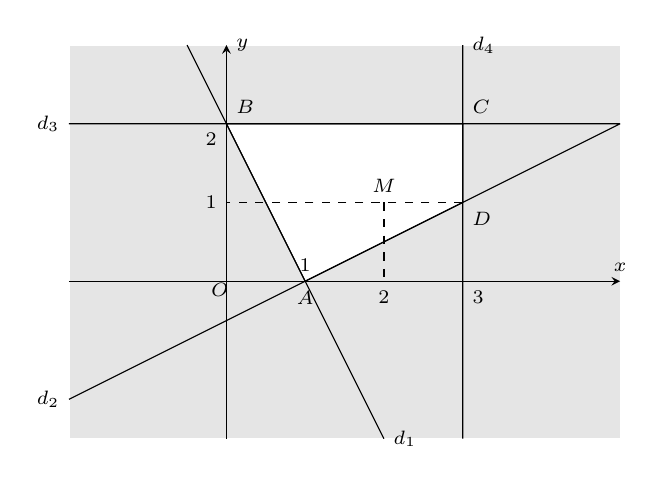
\begin{tikzpicture}[>=stealth]
				\draw[color=white,fill=black!10] (-2,-2) rectangle (5,3);
				\path (-1/2,3) coordinate (A1);
				\path (2,-2) coordinate (B1);
				\path (-2,-3/2) coordinate (A2);
				\path (5,2) coordinate (B2);
				\path (-2,2) coordinate (A3);
				\path (5,2) coordinate (B3);
				\path (3,-2) coordinate (A4);
				\path (3,3) coordinate (B4);
				\path (intersection of A1--B1 and A2--B2) coordinate (A);
				\path (intersection of A1--B1 and A3--B3) coordinate (B);
				\path (intersection of A3--B3 and A4--B4) coordinate (C);
				\path (intersection of A2--B2 and A4--B4) coordinate (D);
				\draw[fill=white] (A) -- (B) -- (C) -- (D) -- cycle;
				\draw[->] (0,-2) -- (0,3) node[right]{\scriptsize $y$};
				\draw[->] (-2,0) -- (5,0) node[above]{\scriptsize $x$};
				\draw (0.15,0.1) node[below left]{\scriptsize $O$};
				\draw (A1) -- (B1) node[right]{\scriptsize $d_1$} (A2)node[left]{\scriptsize $d_2$} -- (B2) (A3)node[left]{\scriptsize $d_3$} -- (B3) (A4) -- (B4) node[right]{\scriptsize $d_4$};
				\draw[dashed] (A) node[above]{\scriptsize $1$} (A) node[below]{\scriptsize $A$} (B) node[below left]{\scriptsize $2$} (B) node[above right]{\scriptsize $B$} (C) node[above right]{\scriptsize $C$} (C|- 0,0) node[below right]{\scriptsize $3$} (D) node[below right]{\scriptsize $D$} -- (D-| 0,0) node[left]{\scriptsize $1$} (2,1) node[above]{\scriptsize $M$} -- (2,0)node[below]{\scriptsize $2$};
			\end{tikzpicture}
		}
	}
\end{vd}

\baitaptl
\begin{bt}%[0D4B4]
	Biểu diễn hình học tập nghiệm của hệ bất phương trình bậc nhất hai ẩn sau
	$$\left\{\begin{aligned}
		x+2y &\geq 1\\
		3x-y & \leq 2 \\
	\end{aligned}\right.$$
	\loigiai{
		\immini{
			Vẽ hai đường thẳng
			\begin{gather*}
				d_1:x+2y=1,\\
				d_2:3x-y=2
			\end{gather*}
			trên cùng một hệ trục tọa độ $Oxy$. Dễ dàng kiểm tra được điểm $O$ thuộc miền nghiệm của cả hai bất phương trình nên ta có miền nghiệm của hệ bất phương trình là miền không bị tô đậm bao gồm cả bờ.
		}{
			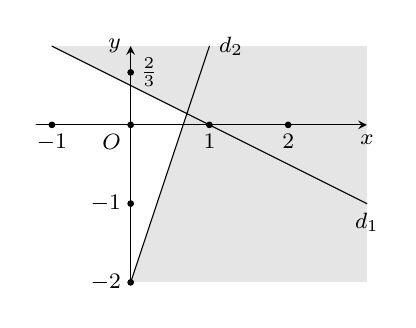
\begin{tikzpicture}[line cap=round, line join=round, font=\footnotesize, >=stealth, scale=1]
				\tikzset{label style/.style={font=\footnotesize}}
				\fill[black!10] (-1,-2) rectangle (3,1);
				\fill[white] (-1,1)--(5/7,1/7)--(0,-2)--(-1,-2)--cycle;
				\draw[->] (-1.2,0)--(3,0) node[below]{$x$};
				\draw[->] (0,-2)--(0,1) node[left]{$y$};
				\draw (-1,1)--(3,-1) node[below]{$d_1$}
				(0,-2)--(1,1) node[right]{$d_2$};
				\draw[fill=black](0,0) circle (1pt) node[below left]{$O$}
				(0,2/3) circle (1pt) node[right]{$\frac{2}{3}$};
				\foreach\x in {-1,1,2} \draw[fill=black] (\x,0) circle (1pt) node[below]{$\x$};
				\foreach\y in {-2,-1} \draw[fill=black] (0,\y) circle (1pt) node[left]{$\y$};
			\end{tikzpicture}	
			
		}
	}
\end{bt}

\begin{bt}%[0D4B4]
	Biểu diễn hình học tập nghiệm của hệ bất phương trình bậc nhất hai ẩn sau
	$$\left\{\begin{aligned}
		x-2y &< 1\\
		x+3y &<-2 \\
		-x+y &<2
	\end{aligned}\right.$$
	\loigiai{
		\immini{
			Vẽ các đường thẳng
			\begin{gather*}
				d_1:x-2y=1\\ d_2:x+2y=-2\\ d_3:-x+y=2
			\end{gather*}
			trên cùng mặt phẳng tọa độ $Oxy$. Ta kiểm tra được điểm $M(-2;-1)$ thuộc miền nghiệm của hệ bất phương trình nên ta có miền nghiệm của hệ bất phương trình là miền trong tam giác $ABC$ không kể các cạch.
		}{
			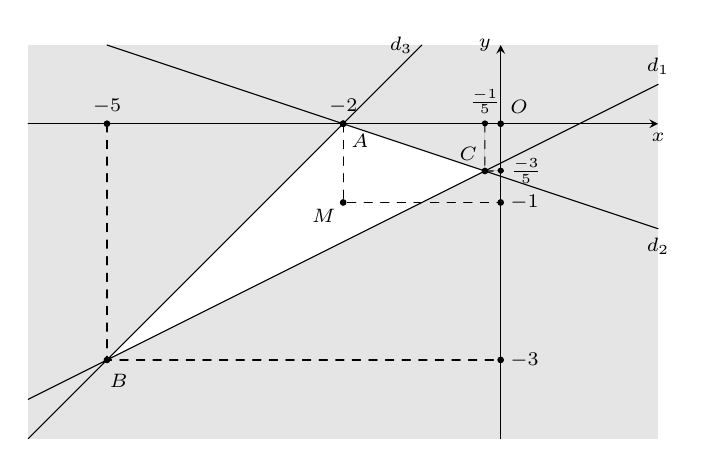
\begin{tikzpicture}[line cap=round, line join=round, font=\scriptsize, >=stealth, scale=1]
				\tikzset{label style/.style={font=\scriptsize}}
				\fill[black!10] (-6,-4) rectangle (2,1);
				\path (-2,0) coordinate (A)
				(-5,-3) coordinate (B)
				(-1/5,-3/5) coordinate (C)
				(-2,-1) coordinate (M);
				\fill[white] (A)--(B)--(C)--cycle;
				\draw[->] (-6,0)--(2,0) node[below]{$x$};
				\draw[->] (0,-4)--(0,1) node[left]{$y$};
				\draw[fill=black] (0,0) circle (1pt) node[above right]{$O$}
				(-5,0) circle (1pt) node[above]{$-5$}
				(-2,0) circle (1pt) node[above]{$-2$}
				(0,-3) circle (1pt) node[right]{$-3$}
				(0,-1) circle (1pt) node[right]{$-1$};
				\draw[smooth] plot[domain=-6:2] (\x,{ \x/2-1/2 }) node[above]{$d_1$}
				plot[domain=-5:2] (\x,{ -\x/3-2/3 }) node[below]{$d_2$}
				plot[domain=-6:-1] (\x,{ \x+2}) node[left]{$d_3$};
				\foreach\x/\y in {A/-45,B/-60,C/135,M/-145} \draw[fill=black] (\x) circle (1pt)+(\y:0.3) node{$\x$};
				\draw[dashed,fill=black] (-1/5,0) circle (1pt) node[above]{$\frac{-1}{5}$}-- (C) (C)--(0,-3/5) circle (1pt) node[right]{$\frac{-3}{5}$};
				\draw[dashed] (-5,0)--(B)--(0,-3)
				(A)--(M)--(0,-1);
			\end{tikzpicture}	
			
		} 
	}
\end{bt}

\begin{bt}%[0D4B4]
	Biểu diễn hình học tập nghiệm của hệ bất phương trình bậc nhất hai ẩn sau
	$$\left\{\begin{aligned}
		3x+y & \leq 5\\
		x+y & \leq 4 \\
		x &\geq 0\\
		y &\geq 0
	\end{aligned}\right.$$
	\loigiai{
		\immini{
			Vẽ các đường thẳng $d_1:3x+y=5$ và $d_2:x+y=4$ lên cùng hệ trục tọa độ. Ta thấy điểm $M(1;1)$ thỏa mãn tất cả các bất phương trình của hệ, do đó tập nghiệm của hệ bất phương trình đã cho là miền trong tứ giác $ABCO$ kể cả các cạnh.
		}{
			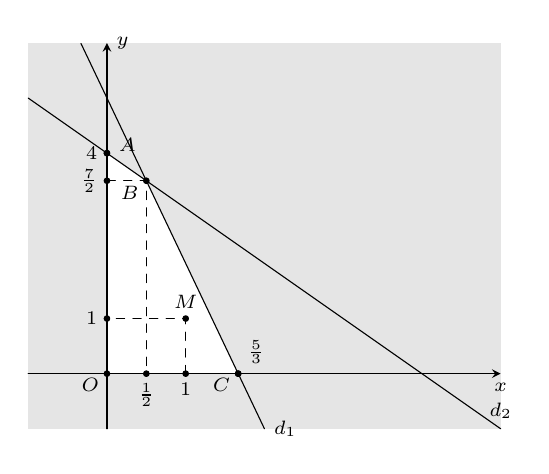
\begin{tikzpicture}[line cap=round, line join=round, font=\scriptsize, >=stealth, scale=1,y=0.7cm]
				\tikzset{label style/.style={font=\footnotesize}}
				\fill[black!10] (-1,-1) rectangle (5,6);
				\path (0,4) coordinate (A)
				(0.5,3.5) coordinate (B)
				(5/3,0) coordinate (C)
				(0,0) coordinate (O)
				(1,1) coordinate (M);
				\fill[white] (A)--(B)--(C)--(O)--cycle;
				\draw[->] (-1,0)--(5,0) node[below]{$x$};
				\draw[->] (0,-1)--(0,6) node[right]{$y$};
				\draw[fill=black]
				(0.5,0) circle (1pt) node[below]{$\frac{1}{2}$}
				(1,0) circle (1pt) node[below]{$1$}
				(5/3,0) circle (1pt) node[above right]{$\frac{5}{3}$}
				(0,3.5) circle (1pt) node[left]{$\frac{7}{2}$}
				(0,1) circle (1pt) node[left]{$1$}
				(0,4) circle (1pt) node[left]{$4$};
				\draw[smooth] plot[domain=-1:5] (\x,{ 4-\x }) node[above]{$d_2$}
				plot[domain=-0.33:2] (\x,{ 5-3*\x }) node[right]{$d_1$};
				\foreach\x/\y in {A/30,B/-135,C/-135,M/90,O/-135} \draw[fill=black] (\x) circle (1pt)+(\y:0.3) node{$\x$};
				\draw[dashed] (0,3.5)--(B)--(0.5,0)
				(1,0)--(M)--(0,1);
			\end{tikzpicture}	
			
		}
	}
\end{bt}

\begin{dang}{Tìm cực trị của biểu thức $F=ax+by$ trên một miền đa giác}
	\begin{enumerate}
		\item Bài toán: \\
		Tìm giá trị lớn nhất, giá trị nhỏ nhất của biểu thức $F=ax+by$ ($a$, $b$ là hai số đã cho không đồng thời bằng $0$) với $x$, $ y$ thỏa mãn hệ bất phương trình bậc nhất hai ẩn (có miền nghiệm là miền đa giác $A_1 A_2 \ldots A_i A_{i+1} \ldots A_n$).
		\item Người ta chứng minh được: Biểu thức $F=ax+by$  có giá trị nhỏ nhất, giá trị lớn nhất tại một trong các đỉnh của đa giác $A_1 A_2 \ldots A_i A_{i+1} \ldots A_n$.
		\item Phương pháp: 
		\begin{itemize}
			\item Bước 1. Tìm miền đa giác $A_1 A_2 \ldots A_i A_{i+1} \ldots A_n$ là miền nghiệm của hệ bất phương trình.
			\item Bước 2. Tìm tọa độ các đỉnh $A_1$, $A_2$, $\ldots$, $A_n$.
			\item Bước 3. Tính $F\left(x_i ; y_i\right)$ trong đó $A_i\left(x_i;y_i\right)$ với $i=1,2,\ldots,\ n$.
			\item Bước 4. Kết luận\\
			Giá trị lớn nhất $M=\max \limits_{i=1,2,\ldots n} F\left(x_i; y_i\right)$.\\
			Giá trị nhỏ nhất $m=\min\limits_{i=1,2,\ldots n} F\left(x_i; y_i\right)$.
		\end{itemize}
	\end{enumerate}
\end{dang}
\viduminhhoa
\begin{vd}%[BG10-2022]%[Toanvo]%[0D4G4-4]
	Cho cặp số $\left(x;y\right)$  là nghiệm của hệ  $\heva{&3x-y \geq -1\\&2x+y \leq 6\\&x+3y>3}$. Tìm giá trị lớn nhất và nhỏ nhất của biểu thức $f\left(x;y\right)=2x-3y+1$.
	\loigiai{
		\begin{itemize}
			\item Trước hết ta biểu diễn miền nghiệm của hệ (*):
			\begin{itemize}
				\item  Vẽ các đường thẳng $d_1 \colon 3x-y=-1$; $d_2 \colon 2x+y=6$; $d_3 \colon x+3y=3$.
				\item  Điểm $M(1;1)$ có tọa độ thỏa mãn tất cả các bất phương trình trong hệ nên ta tô đậm các nửa mặt phẳng bờ $d_1;d_2;d_3$ không chứa điểm $M$. Miền không bị tô đậm là hình tam giác $ABC$, tính cả ba cạnh $AB,BC,CA$ trong hình vẽ dưới là miền nghiệm của hệ bất phương trình đã cho.
			\end{itemize}
			\begin{center}
				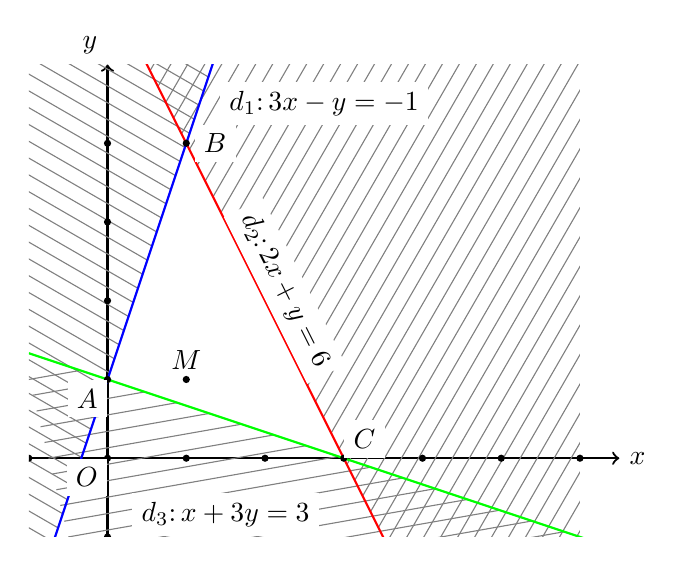
\begin{tikzpicture}
					\draw[->,line width=0.8pt] (-1,0)--(6.5,0) node[right]{$x$};
					\draw[->,line width=0.8pt] (0,-1)--(0,5) node[above left]{$y$};
					
					\clip (-1,-1) rectangle (6.5,5);
					
					
					\begin{scope}
						\clip (-2,-5)--(-2,7)--(2,7)--(-2,-5);
						\foreach \x in {-1,-.85,...,20}{
							\pgfmathsetmacro{\y}{-2*\x+8}
							\draw[gray] (\x,\y)--++(150:10);
						}			
					\end{scope}
					
					\begin{scope}
						\clip (-2,10)--(6,10)--(6,-6)--(-2,10);
						\foreach \x in {-1,-.9,...,20}{
							\pgfmathsetmacro{\y}{-2*\x+1}
							\draw[gray] (\x,\y)--++(1500:10);
						}			
					\end{scope}
					
					\pgfmathsetmacro{\hsgg}{-1/3}
					\begin{scope}
						\clip (-3,2)--(-3,-3)--(12,-3)--(-3,2);
						\foreach \x in {-1,-.95,...,20}{
							\pgfmathsetmacro{\y}{-4*\x-3}
							\draw[gray] (\x,\y)--++(10:10);
						}			
					\end{scope}
					
					
					
					\draw[thick,smooth,domain=-1:6.5,blue] plot (\x,{3*\x+1});
					\draw[thick,smooth,domain=-1:6.5,red] plot (\x,{-2*\x+6});
					\draw[thick,smooth,domain=-1:6.5,green] plot (\x,{\hsgg*\x+1});
					
					\path (2.5,4.5)--(3,4.5) node[fill=white,pos=.5,sloped]{$d_{1} \colon 3x-y=-1$};
					\path (1,4)--(3,0) node[fill=white,pos=.5,sloped,above]{$d_{2} \colon 2x+y=6$};
					\path (1,-1)--(2,-1) node[fill=white,pos=.5,sloped,above]{$d_{3} \colon x+3y=3$};
					
					\foreach \i in {-1,1,2,3,4}{
						\fill (0,\i) circle (1.3pt);
					}
					\foreach \i in {-1,0,1,2,3,4,5,6}{
						\fill (\i,0) circle (1.3pt);
					}
					\fill (1,1) circle (1.3pt) (1,4) circle (1.3pt);
					
					\path 
					(0,1) node[below left,fill=white]{$A$}
					(1,1) node[above]{$M$}
					(3,0) node[above right,fill=white]{$C$}
					(1.1,4) node[right,fill=white]{$B$}
					(0,0) node[below left,fill=white]{$O$};
				\end{tikzpicture}
			\end{center}
			\item Tìm tọa độ các điểm $A,B,C$:
			\begin{itemize}
				\item $A=d_1 \cap d_3$ nên tọa độ thỏa mãn $\heva{	&3x-y=-1\\
					&x+3y=3} \Leftrightarrow \heva{&x=0\\
					&y=1}$. Vậy $A(0;1)$.
				\item  $B=d_1 \cap d_2$ nên tọa độ thỏa mãn $\heva{&3x-y=-1\\
					&2x+y=6} \Leftrightarrow \heva{&x=1\\
					&y=4} $. Vậy $B(1;4)$.
				\item $C=d_2 \cap d_3$ nên tọa độ thỏa mãn $\heva{&2x+y=6\\
					&x+3y=3}\Leftrightarrow \heva{&x=3\\
					&y=0} $. Vậy $C(3;0)$.
			\end{itemize}
		\end{itemize}
		Tính giá trị của $f(x;y)=2x-3y+1$ tại tất cả các đỉnh của tam giác $ABC$: 
		\begin{center}
			\begin{tabular}{|p{5cm}||p{2cm}|p{2cm}|p{2cm}|}
				\hline
				$(x;y)$ & $A(0;1)$ & $B(1;4)$ & $C(3;0)$ \\
				\hline
				$f(x;y)=2x-3y+1$  & $-2$  & $-9$ & $7$ \\
				\hline
			\end{tabular}
		\end{center}
		Suy ra $\min f(x;y)=f(1;4)=-9$ và $\max f(x;y)=f(3;0)=7$.\\
		
	}
\end{vd}
\begin{vd}%[BG10-2022]%[Toanvo]%[0D4G4-4]
	Quảng cáo sản phẩm trên truyền hình là một hoạt động quan trọng trong kinh doanh của các doanh nghiệp.\\
	Theo Thông báo số $10/2019$, giá quảng cáo trên VTV1 là $30$ triệu đồng cho $15$ giây/$1$ lần quảng cáo vào khoảng $20$h$30$; là $6$ triệu đồng cho $15$ giây/$1$ lần quảng cáo vào khung giờ $16$h$00-17$h$00$.\\
	Một công ty dự định chi không quá $900$ triệu đồng để quảng cáo trên VTV1 với yêu cầu quảng cáo về số lần phát như sau: ít nhất $10$ lần quảng cáo vào khoảng
	$20$h$30$ và không quá $50$ lần quảng cáo vào khung giờ $16$h$00-17$h$00$. 
	\loigiai{
		Gọi $x, \,y$ lần lượt là số lần phát quảng cáo vào khoảng $20$h$30$  và vào khung giờ $16$h$00-17$h$00$. Theo giả thiết, ta có: $x \in \mathbb{N},\, y \in \mathbb{N},\, x \geq 10,0 \leq y \leq 50$.\\
		Tổng số lần phát quảng cáo là $T=x+y$.\\
		Số tiền công ty cần chi là $30 x+6 y$ (triệu đồng).\\
		Do công ty dự định chi không quá $900$ triệu đồng nên $30 x+6 y \leq 900$ hay $5 x+y \leq 150$.\\
		Ta có hệ bất phương trình: $\heva{5 x+y \leq 150 \\ x \geq 10 \\ 0 \leq y \leq 50.} $ \hfill(I)	
		Bài toán đưa về tìm $x, y$ là nghiệm của hệ bất phương trình (I) sao cho $T=x+y$ có giá trị lớn nhất.\\
		Trước hết, ta xác định miền nghiệm của hệ bất phương trình (I).\\
		Miền nghiệm của hệ bất phương trình (I) là miền tứ giác $A B C D$ với $A(30 ; 0), B(20 ; 50)$, $C(10 ; 50), D(10 ; 0)$ (Hình vẽ).
		\immini{
			Người ta chứng minh được: Biểu thức $T=x+y$ đạt được giá trị lớn nhất tại một trong các đỉnh của tứ giác $A B C D$.
			Tính giá trị của biểu thức $T=x+y$ tại cặp số $(x ; y)$ là toạ độ các đỉnh của tứ giác $A B C D$ rồi so sánh các giá trị đó. Ta được $T$ đạt giá trị lớn nhất khi $x=20, y=50$ ứng với tọa độ đỉnh $B$.\\
			Vậy để phát được số lần quảng cáo nhiều nhất thì số lần phát quảng cáo vào khoảng $20$h$30$  và vào khung giờ $16$h$00-17$h$00$  lần lượt là $20$ và $50$ lần.
		}{\begin{tikzpicture}[scale=0.07,line join=round, line cap=round,>=stealth,thick]
				\tikzset{label style/.style={font=\footnotesize}}
				\begin{scope}
					
					\clip (-20,-20) rectangle (60,60);
					\fill[pattern=crosshatch dots] (-21,255)--(61,255)--(61,-155)--cycle;
					\fill[pattern=crosshatch dots] (10,-20)--(-20,-20)--(-20,60)--(10,60)--cycle;
					\fill[pattern=crosshatch dots] (-20,0)--(-20,-20)--(60,-20)--(60,0)--cycle;
					\fill[pattern=crosshatch dots] (-20,50)--(-20,60)--(60,60)--(60,50)--cycle;
					\draw (18,60)--(34,-20) ;
					\draw (10,-20)--(10,60) ;
					\draw (-20,50)--(60,50) ;
				\end{scope}
				\draw[->] (-20,0)--(60,0) node[below]{$x$};
				\draw[->] (0,-20)--(0,60) node[left]{$y$};
				\draw (0,0) node[below left]{$O$};
				\path (10,50) coordinate(C) (10,0) coordinate(D) (30,0) coordinate(A) (20,50) coordinate(B);
				\foreach \i in {A,B,C,D} \fill (\i) circle(20pt) ($(\i)+(55:5)$)node{$\i$};
				\foreach \x in {10,20,30}
				\draw[thin] (\x,1pt)--(\x,-1pt) node [below right] {$\x$};
				\foreach \y in {50}
				\draw[thin] (1pt,\y)--(-1pt,\y) node [below left] {$\y$};
		\end{tikzpicture}}
	}
\end{vd}
\begin{vd}%[BG10-2022]%[Toanvo]%[0D4G4-4]
	Một hộ nông dân dự định trồng đậu và cà trên diện tích $8$ ha. Nếu trồng đậu thì cần $20$ công và thu $3$ triệu đồng trên diện tích mỗi ha, nếu trồng cà thì cần $30$ công và thu $4$ triệu đồng trên diện tích mỗi ha. Hỏi cần trồng mỗi loại cây trên với diện tích là bao nhiêu để thu về được nhiều tiền nhất, biết rằng tổng số công không quá $180$.
	\loigiai{
		Gọi diện tích để trồng đậu là $x$ (ha); diện tích để trồng cà là  $y$ (ha). ( điều kiện: $0 \leq x,y \leq 8$ ).\\
		Tổng số diện tích sử dụng là $x+y$.\\
		Tổng số công cần sử dụng là $20x+30y$. \\
		Ta có hệ bất phương trình
		$$\heva{&0\leq x\leq8\\&0\leq y\leq8\\&x+y\leq8\\&20x+30y\leq180}\Leftrightarrow\heva{&0\leq x\leq8\\&0\leq y\leq8\\&x+y\leq8\\&2x+3y\leq18.}$$
		Vẽ các đường thẳng thẳng $(d_1) \colon x+y=8,\ (d_2) \colon 2x+3y=18,\ (d_3) \colon x=8,\ (d_4) \colon y=8$ ta được miền
		nghiệm của hệ bất phương trình là phần tô đậm như hình vẽ
		\begin{center}
			\begin{tikzpicture}[line join = round, line cap = round, >=stealth, font=\footnotesize, scale=.5]
				\tikzset{label style/.style={font=\footnotesize}}
				\def \xmin{-6}
				\def \xmax{15}
				\def \ymin{-5}
				\def \ymax{14}
				\tkzDefPoints{0/6/A, 6/2/B, 8/0/C, 0/0/D, 0/8/E, 9/0/F, 8/8/G}
				\draw[gray!20](\xmin,\ymin) grid (\xmax,\ymax);
				\draw [->](\xmin,0)--(0,0)node[below left]{$O$}--(\xmax,0)node[above]{$x$};
				\draw [->](0,\ymin)--(0,\ymax)node[right]{$y$};
				\foreach \x in {-5,5,10} \draw[shift={(\x,0)}] (0pt,2pt)--(0pt,-2pt) node[below]{$\x$};
				\foreach \y in {5,10} \draw [shift={(0,\y)}] (2pt,0pt)--(-2pt,0pt) node[left]{$\y$};
				\tkzDrawLines[add=0.5 and 0.5](E,C A,F C,G E,G)
				\tkzDrawPoints[fill=black](A,B,C,D)
				\tkzLabelPoints[right](A)
				\tkzLabelPoints[above](B)
				\tkzLabelPoints[below left](C)
				\tkzLabelPoints[below right](D)
				\tkzFillPolygon[color=cyan,fill opacity=.5](A,B,C,D)
				\tkzLabelLine[pos=1.7,above right](B,E){$(d_1)$}
				\tkzLabelLine[pos=1.8,above right](B,A){$(d_2)$}
				\tkzLabelLine[pos=1.5,right](C,G){$(d_3)$}
				\tkzLabelLine[pos=1.5,above](E,G){$(d_4)$}
			\end{tikzpicture}
		\end{center}
		Ta có 
		{\allowdisplaybreaks
			\begin{eqnarray*}
				&&A(0;6)=(d_2) \cap Oy,B(6;2)=(d_1) \cap (d_2)\\
				&&C(8;0)=(d_1) \cap Ox,D \equiv O(0;0).
			\end{eqnarray*}
		}
		Số tiền thu về là $f(x;y)=3x+4y$ (triệu đồng).
		\begin{center}
			\renewcommand\arraystretch{1.6}
			\renewcommand{\tabcolsep}{6mm}
			\begin{tabular}{|c|c|c|c|c|}
				\hline 
				$M(x;y)$& $A$ & $B$ & $C$ & $D$ \\ 
				\hline 
				$f(x,y)=3x+4y$& $24$ & $26$ & $24$ & $0$ \\ 
				\hline 
			\end{tabular} 
		\end{center}
		Do đó $f(x,y)$ đạt giá trị lớn nhất tại $B(6;2)$.\\
		Vậy để thu được nhiều tiền nhất thì cần trồng 6 ha đậu và 2 ha cà.
	}	
\end{vd}
\baitaptl
\begin{bt}%[BG10-2022]%[Toanvo]%[0D4G4-4]
	Một gia đình cần ít nhất $900$ đơn vị protein và $400$ đơn vị lipit trong thức ăn mỗi ngày. Mỗi kg thịt bò chứa $800$ đơn vị protein và $200$ đơn vị lipit. Mỗi kg thịt lợn chứa $600$ đơn vị protein và $400$ đơn vị lipit. Biết rằng mỗi ngày gia đình này chỉ mua tối đa $1{,}5$ kg thịt bò và $1$ kg thịt lợn, giá tiền $1$ kg thịt bò là $200$ nghìn đồng, $1$ kg thịt lợn là $100$ nghìn đồng. Hỏi gia đình đó phải mua bao nhiêu kg thịt mỗi loại để số tiền bỏ ra là ít nhất.
	\loigiai{
		Gọi số kg thịt bò cần mua là $x$ (kg); số kg thịt lợn cần mua là $y$ (kg). Điều kiện: $0 \leq x \leq 1{,}5, 0 \leq y \leq 1$.\\
		Khi đó số đơn vị protein là $800x+600y$.\\
		Số đơn vị lipit là $200x+400y$.\\
		Ta có hệ bất phương trình $$\heva{&0\leq x\leq 1{,}5\\&0\leq y\leq 1\\&800x+600y\geq 900\\&200x+400y\geq200}\Leftrightarrow\heva{&0\leq x\leq 1{,}5\\&0\leq y\leq 1\\&8x+6y\geq9\\&x+2y\geq2.}$$	
		Vẽ các đường thẳng $(d_1)\colon x=1{,}5$, $(d_2)\colon y=1$, $(d_3)\colon 8x+6y=9$, $(d_4)\colon x+2y=2$. Ta được miền nghiệm của hệ bất phương trình là phần tô đậm trong hình vẽ.
		\begin{center}
			\begin{tikzpicture}[line join = round, line cap = round, >=stealth, font=\footnotesize, scale=1.2]
				\tikzset{label style/.style={font=\footnotesize}}
				\def \xmin{-3.5}
				\def \xmax{5.5}
				\def \ymin{-1.5}
				\def \ymax{6}
				\tkzDefPoints{0.375/1/A, 1.5/1/B, 1.5/0.25/C, 0.6/0.7/D}
				\draw[gray!20](\xmin,\ymin) grid (\xmax,\ymax);
				\draw [->](\xmin,0)--(0,0)node[below left]{$O$}--(\xmax,0)node[above]{$x$};
				\draw [->](0,\ymin)--(0,\ymax)node[right]{$y$};
				\foreach \x in {-3,-2,-1,1,2,3,4,5} \draw[shift={(\x,0)}] (0pt,2pt)--(0pt,-2pt) node[below]{$\x$};
				\foreach \y in {-1,2,3,4,5} \draw [shift={(0,\y)}] (2pt,0pt)--(-2pt,0pt) node[left]{$\y$};
				\draw [shift={(0,1)}] (2pt,0pt)--(-2pt,0pt) node[below left]{$1$};
				\tkzDrawLine[add=6 and 2](B,C)
				%\tkzDrawLine[add=0.5 and 0.5](B,C A,B A,D D,C)
				\tkzDrawLine[add=3 and 3](A,B)
				\tkzDrawLine[add=12 and 6](A,D)
				\tkzDrawLines[add=4 and 2](D,C)
				\tkzDrawPoints[fill=black](A,B,C,D)
				\tkzLabelPoints[above right](A,B,C)
				\tkzLabelPoints[below](D)
				\tkzFillPolygon[color=cyan,fill opacity=.5](A,B,C,D)
				\tkzLabelLine[pos=7,right](C,B){$(d_1)$}
				\tkzLabelLine[pos=3.5,above right](A,B){$(d_2)$}
				\tkzLabelLine[pos=12,above right](D,A){$(d_3)$}
				\tkzLabelLine[pos=5,above right](C,D){$(d_4)$}
			\end{tikzpicture}
		\end{center}
		Ta có 
		{\allowdisplaybreaks
			\begin{eqnarray*}
				&&A\left(\dfrac{3}{8};1\right)=(d_3) \cap (d_2), B(1{,}5;1)=(d_1) \cap (d_2),\\
				&&C(1{,}5;0{,}25)=(d_1) \cap (d_4), D\left(\dfrac{3}{5};\dfrac{7}{10}\right)=(d_3) \cap (d_4).
			\end{eqnarray*}
		}
		Số tiền bỏ ra là $f(x,y)=200x+100y$ (nghìn đồng).
		\begin{center}
			\renewcommand\arraystretch{1.6}
			\renewcommand{\tabcolsep}{6mm}
			\begin{tabular}{|c|c|c|c|c|}
				\hline 
				$M(x;y)$& $A$ & $B$ & $C$ & $D$ \\ 
				\hline 
				$f(x,y)=200x+100y$& $175$ & $400$ & $325$ & $190$ \\ 
				\hline 
			\end{tabular} 
		\end{center}
		Do đó $f(x,y)$ đạt giá trị nhỏ nhất tại $A\left(\dfrac{3}{8};1\right)$.\\
		Vậy để số tiền bỏ ra nhỏ nhất thì cần mua $\dfrac{3}{8}$ kg thịt bò và $1$ kg thịt lợn.
	}
\end{bt}
\begin{bt}%[BG10-2022]%[Toanvo]%[0D4G4-4]
	Người ta định dùng hai loại nguyên liệu để chiết xuất ít nhất $120$ kg hóa chất $A$ và $9$ kg hóa chất $B$. Từ mỗi tấn nguyên liệu loại I giá $4$ triệu đồng có thể chiết xuất được $20$ kg chất $A$ và $0{,}6$ kg chất $B$. Từ mỗi tấn nguyên liệu loại II giá $3$ triệu đồng có thể chiết xuất được $10$ kg chất $A$ và $1{,}5$ kg chất $B$. Hỏi phải dùng bao nhiêu tấn nguyên liệu mỗi loại để chi phí mua nguyên liệu là ít nhất. Biết rằng cơ sở cung cấp nguyên liệu chỉ có thể cung cấp không quá $10$ tấn nguyên liệu loại I và không quá $9$ tấn nguyên liệu loại II. 
	\loigiai{
		Gọi số tấn nguyên liệu loại I cần sử dụng là $x$ (tấn); số tấn nguyên liệu loại II cần sử dụng là  $y$ (tấn).\\
		Điều kiện: $0 \leq x \leq 10$, $0 \leq y \leq 9$.\\
		Khi đó số kg chất $A$ thu được là $20x+10y$, số kg chất $B$ thu được là $0{,}6x+1{,}5y$.\\
		Ta có hệ bất phương trình $$\heva{&0\leq x\leq 10\\&0\leq y\leq 9\\&20x+10y\geq120\\&0{,}6x+1{,}5y\geq9}\Leftrightarrow \heva{&0\leq x \leq10\\&0\leq y \leq 9\\&2x+y\geq 12\\&2x+5y\geq30.}$$
		Vẽ các đường thẳng $(d_1) \colon x=10$, $(d_2) \colon y=9$, $(d_3) \colon 2x+y=12$, $(d_4) \colon 2x+5y=30$. \\
		Ta có miền nghiệm của hệ bất phương trình là phần tô màu như hình vẽ:
		\begin{center}
			\begin{tikzpicture}[line join = round, line cap = round, >=stealth, font=\footnotesize, scale=.5]
				\tikzset{label style/.style={font=\footnotesize}}
				\def \xmin{-8}
				\def \xmax{17}
				\def \ymin{-5}
				\def \ymax{15}
				\tkzDefPoints{1.5/9/A, 10/9/B, 10/2/C, 3.75/4.5/D}
				\draw[gray!20](\xmin,\ymin) grid (\xmax,\ymax);
				\draw [->](\xmin,0)--(0,0)node[below left]{$O$}--(\xmax,0)node[above]{$x$};
				\draw [->](0,\ymin)--(0,\ymax)node[right]{$y$};
				\foreach \x in {-5,5,15} \draw[shift={(\x,0)}] (0pt,2pt)--(0pt,-2pt) node[below]{$\x$};
				\draw[shift={(10,0)}] (0pt,2pt)--(0pt,-2pt) node[below left]{$10$};
				\foreach \y in {5,10} \draw [shift={(0,\y)}] (2pt,0pt)--(-2pt,0pt) node[left]{$\y$};
				\tkzDrawLine[add=.8 and .8](C,B)
				\tkzDrawLine[add=.8 and .5](A,B)
				\tkzDrawLine[add=2 and 1.2](D,A)
				\tkzDrawLines[add=1 and 1.5](C,D)
				\tkzDrawPoints[fill=black](A,B,C,D)
				\tkzLabelPoints[above right](A,B,C)
				\tkzLabelPoints[below](D)
				\tkzFillPolygon[color=cyan,fill opacity=.5](A,B,C,D)
				\tkzLabelLine[pos=1.7,right](C,B){$(d_1)$}
				\tkzLabelLine[pos=1.3,above right](A,B){$(d_2)$}
				\tkzLabelLine[pos=2.2,below left](D,A){$(d_3)$}
				\tkzLabelLine[pos=2.4,below left](C,D){$(d_4)$}
			\end{tikzpicture}
		\end{center}
		Ta có 
		{\allowdisplaybreaks
			\begin{eqnarray*}
				&&(d_2) \cap (d_3)=A\left(\dfrac{3}{2};9\right),\ (d_2) \cap (d_1)=B(10;9),\\
				&&(d_1) \cap (d_4)=C(10;2),\ (d_4) \cap (d_3)=D\left(\dfrac{15}{4};\dfrac{9}{2}\right).
			\end{eqnarray*}
		}
		Chi phí mua nguyên liệu cần bỏ ra là $f(x,y)=4x+3y$ (triệu đồng).
		\begin{center}
			\renewcommand\arraystretch{1.6}
			\renewcommand{\tabcolsep}{6mm}
			\begin{tabular}{|c|c|c|c|c|}
				\hline 
				$M(x;y)$& $A$ & $B$ & $C$ & $D$ \\ 
				\hline 
				$f(x,y)=4x+3y$& $3$ & $67$ & $46$ & $28{,}5$ \\
				\hline 
			\end{tabular} 
		\end{center}
		Do đó $f(x,y)$ đạt giá trị nhỏ nhất tại $D\left(\dfrac{15}{4};\dfrac{9}{2}\right)$.\\
		Vậy để chi phí nguyên liệu là ít nhất ta cần sử dụng $\dfrac{15}{4}=3{,}75$ tấn nguyên liệu loại I và $\dfrac{9}{2}=4{,}5$ tấn nguyên liệu loại II.
	}
\end{bt}
\begin{bt}%[BG10-2022]%[Toanvo]%[0D4G4-4]
	Có ba nhóm máy $A$, $B$, $C$ dùng để sản xuất ra hai loại sản phẩm I và II. Để sản xuất một đơn vị sản phẩm mỗi loại phải lần lượt dùng các máy thuộc các nhóm khác nhau. Số máy trong một nhóm và số máy của từng nhóm cần thiết để sản xuất ra một đơn vị sản phẩm thuộc mỗi loại  được cho trong bảng sau:
	\begin{center}
		\begin{tabular}{|c|c|p{2.5cm}|p{2.5cm}|}
			\hline 
			\multirow{2}{*}{Nhóm}& \multirow{2}{*}{Số máy trong mỗi nhóm}  & \multicolumn{2}{p{5cm}|}{Số máy trong từng nhóm để sản xuất ra một đơn vị sản phẩm} \\ 
			\cline{3-4} 
			&  & Loại I & Loại II  \\ 
			\hline 
			A & 10 & 2 & 2 \\ 
			\hline 
			B & 4 & 0 & 2 \\ 
			\hline 
			C & 12 & 2 & 4 \\ 
			\hline 
		\end{tabular} 
	\end{center}
	Một đơn vị sản phẩm I lãi ba nghìn đồng, một đơn vị sản phẩm loại II lãi năm nghìn đồng. Hãy lập phương án để việc sản xuất hai loại sản phẩm trên có lãi cao nhất. 
	\loigiai{
		Gọi số sản phẩm loại I cần sản xuất là $x$; số sản phẩm loại II cần sản xuất là $y$. Điều kiện: $x,y \geq 0$.\\
		Số máy nhóm $A$ cần sử dụng là $2x+2y$.\\
		Số máy nhóm $B$ cần sử dụng là $2y$.\\
		Số máy nhóm $C$ cần sử dụng là $2x+4y$.\\
		Ta có hệ bất phương trình $$\heva{&x\geq0\\&y\geq0\\&2x+2y\leq10\\&2y\leq4\\&x+2y\leq6}\Leftrightarrow\heva{&x\geq0\\&0\leq y \leq 2\\&x+y\leq5\\&x+2y\leq6.}$$
		Vẽ các đường thẳng $(d_1) \colon y=2$, $(d_2) \colon x+y=5$, $(d_3) \colon x+2y=6$. Ta có miền nghiệm của bất phương trình là phần tô màu như hình vẽ:
		\begin{center}
			\begin{tikzpicture}[line join = round, line cap = round, >=stealth, font=\footnotesize, scale=1.2]
				\tikzset{label style/.style={font=\footnotesize}}
				\def \xmin{-2.5}
				\def \xmax{8}
				\def \ymin{-2}
				\def \ymax{6.5}
				\tkzDefPoints{0/2/A, 2/2/B, 4/1/C, 5/0/D, 0/0/E}
				\draw[gray!20](\xmin,\ymin) grid (\xmax,\ymax);
				\draw [->](\xmin,0)--(0,0)node[below left]{$O$}--(\xmax,0)node[above]{$x$};
				\draw [->](0,\ymin)--(0,\ymax)node[right]{$y$};
				\foreach \x in {-2,-1,1,2,3,4,5,6,7} \draw[shift={(\x,0)}] (0pt,2pt)--(0pt,-2pt) node[below]{$\x$};
				\foreach \y in {-1,1,3,4,5,6} \draw [shift={(0,\y)}] (2pt,0pt)--(-2pt,0pt) node[left]{$\y$};
				\draw [shift={(0,2)}] (2pt,0pt)--(-2pt,0pt) node[below left]{$2$};
				\tkzDrawLine[add=1 and 2.7](A,B)
				%\tkzDrawLine[add=0.5 and 0.5](B,C A,B A,D D,C)
				\tkzDrawLine[add=1.5 and 5](D,C)
				\tkzDrawLine[add=2 and 2](C,B)
				%\tkzDrawLines[add=4 and 2](D,C)
				\tkzDrawPoints[fill=black](A,B,C,D,E)
				\tkzLabelPoints[above right](A,B,C,D)
				%\tkzLabelPoints[below](D)
				\tkzLabelPoints[below right](E)
				\tkzFillPolygon[color=cyan,fill opacity=.5](A,B,C,D,E)
				\tkzLabelLine[pos=3.6,above](A,B){$(d_1)$}
				\tkzLabelLine[pos=6,below left](D,C){$(d_2)$}
				\tkzLabelLine[pos=3,below left](C,B){$(d_3)$}
				%\tkzLabelLine[pos=5,above right](C,D){$(d_4)$}
			\end{tikzpicture}
		\end{center} 
		Ta có 
		{\allowdisplaybreaks
			\begin{eqnarray*}
				&&(d_1) \cap Oy=A(0;2), (d_1) \cap (d_3)=B(2;2), (d_2)\cap (d_3)=C(4;1)\\
				&&(d_2) \cap Ox=D(5;0), E \equiv O=(0;0). 
			\end{eqnarray*}
		}
		Lãi suất thu được là $f(x,y)=3x+5y$ (nghìn đồng).
		\begin{center}
			\renewcommand\arraystretch{1.6}
			\renewcommand{\tabcolsep}{6mm}
			\begin{tabular}{|c|c|c|c|c|c|}
				\hline 
				$M(x;y)$& $A$ & $B$ & $C$ & $D$ & $E$ \\ 
				\hline 
				$f(x,y)=3x+5y$& $10$ & $16$ & $17$ & $15$ & $0$ \\
				\hline 
			\end{tabular} 
		\end{center}
		Do đó $f(x,y)$ đạt giá trị lớn nhất tại $C(4;1)$.\\
		Vậy phương án sản xuất 4 sản phẩm loại I và $1$ sản phẩm loại II sẽ cho lãi cao nhất.
	}
\end{bt}
\begin{bt}%[BG10-2022]%[Toanvo]%[0D4G4-4]
	Một nhà khoa học nghiên cứu về tác động phối hợp của vitamin $A$ và vitamin $B$ đối với cơ thể con người. Kết quả như sau:
	\begin{enumerate}
		\item  Một người có thể tiếp nhận được mỗi ngày không quá $600$ đơn vị vitamin $A$ và không quá $500$ đơn vị vitamin $B$.
		\item Một người mỗi ngày cần từ $400$ đến $1000$ đơn vị vitamin cả $A$ lẫn $B$.
		\item  Do tác động phối hợp của hai loại vitamin, mỗi ngày số đơn vị vitamin $B$ phải nhiều hơn $\dfrac{1}{2}$ số đơn vị vitamin $A$ nhưng không nhiều hơn ba lần số đơn vị vitamin $A$. Biết giá một đơn vị vitamin $A$ là $9$ đồng và giá một đơn vị vitamin $B$ là $7{,}5$ đồng.
	\end{enumerate}
	Tìm phương án dùng vitamin $A$ và vitamin $B$ thỏa mãn các điều kiện trên sao cho số tiền phải trả ít nhất.
	\loigiai{
		Gọi số đơn vị vitamin $A$ cần dùng là $x$; số đơn vị vitamin $B$ cần dùng là $y$.\\
		Điều kiện: $0 \leq x \leq 600$, $0 \leq y \leq 500$.\\
		Tổng số đơn vị vitamin $A$ và vitamin $B$ cần dùng là $x+y$.\\
		Ta có hệ bất phương trình $\heva{&0\leq x\leq 600\\&0\leq y\leq 500\\&400\leq x+y\leq 1000\\&\dfrac{x}{2}\leq y\leq 3x.}$\\
		Vẽ các đường thẳng $(d_1) \colon x=600$, $(d_2) \colon y=500$, $(d_3) \colon x+y=400$, $(d_4) \colon x+y=1000$, \\
		$(d_5) \colon \dfrac{x}{2}-y=0$, $(d_6) \colon y=3x$.\\
		Ta có miền nghiệm của hệ bất phương trình như hình vẽ:
		\begin{center}
			\begin{tikzpicture}[line join = round, line cap = round, >=stealth, font=\footnotesize, scale=1.2]
				\tikzset{label style/.style={font=\footnotesize}}
				\def \xmin{-3.5}
				\def \xmax{5.5}
				\def \ymin{-1}
				\def \ymax{6}
				\tkzDefPoints{0.833333/2.5/A, 2.5/2.5/B, 3/2/C, 3/1.5/D, 1.33333/0.66666/E, 0.5/1.5/F}
				\draw[gray!20](\xmin,\ymin) grid (\xmax,\ymax);
				\draw [->](\xmin,0)--(0,0)node[above left]{$O$}--(\xmax,0)node[above]{$x$};
				\draw [->](0,\ymin)--(0,\ymax)node[right]{$y$};
				\draw[shift={(-3,0)}] (0pt,2pt)--(0pt,-2pt) node[below]{$-600$};
				\draw[shift={(-2,0)}] (0pt,2pt)--(0pt,-2pt) node[below]{$-400$};
				\draw[shift={(-1,0)}] (0pt,2pt)--(0pt,-2pt) node[below]{$-200$};
				\draw[shift={(1,0)}] (0pt,2pt)--(0pt,-2pt) node[below]{$200$};
				\draw[shift={(2,0)}] (0pt,2pt)--(0pt,-2pt) node[below]{$400$};
				\draw[shift={(3,0)}] (0pt,2pt)--(0pt,-2pt) node[below right]{$600$};
				\draw[shift={(4,0)}] (0pt,2pt)--(0pt,-2pt) node[below]{$800$};
				\draw[shift={(5,0)}] (0pt,2pt)--(0pt,-2pt) node[below]{$1000$};
				\draw[shift={(0,1)}] (2pt,0pt)--(-2pt,0pt) node[left]{$200$};
				\draw[shift={(0,2)}] (2pt,0pt)--(-2pt,0pt) node[left]{$400$};
				\draw[shift={(0,3)}] (2pt,0pt)--(-2pt,0pt) node[left]{$600$};
				\draw[shift={(0,4)}] (2pt,0pt)--(-2pt,0pt) node[left]{$800$};
				\draw[shift={(0,5)}] (2pt,0pt)--(-2pt,0pt) node[left]{$1000$};
				\tkzDrawLine[add=4 and 7](D,C)
				\tkzDrawLine[add=1.5 and 2](B,A)
				\tkzDrawLine[add=1.6 and 4](E,F)
				\tkzDrawLines[add=4.5 and 6](C,B)
				\tkzDrawLines[add=1.7 and 1](E,D)
				\tkzDrawLines[add=2.2 and 3](F,A)
				\tkzDrawPoints[fill=black](A,B,C,D,E,F)
				\tkzLabelPoints[above right](A,B,C)
				\tkzLabelPoints[below right](D)
				\tkzLabelPoints[below](E)
				\tkzLabelPoints[left](F)
				\tkzFillPolygon[color=cyan,fill opacity=.5](A,B,C,D,E,F)
				\tkzLabelLine[pos=7.5,right](D,C){$(d_1)$}
				\tkzLabelLine[pos=3,above](B,A){$(d_2)$}
				\tkzLabelLine[pos=5,above right](E,F){$(d_3)$}
				\tkzLabelLine[pos=7,above](C,B){$(d_4)$}
				\tkzLabelLine[pos=2,below](E,D){$(d_5)$}
				\tkzLabelLine[pos=4,left](F,A){$(d_6)$}
			\end{tikzpicture}
		\end{center} 
		Ta có 
		{\allowdisplaybreaks
			\begin{eqnarray*}
				&&(d_1) \cap (d_6)=A\left(\dfrac{500}{3};500\right), (d_4) \cap (d_2)=B(500;500), (d_1) \cap (d_4)=C(600;400),\\
				&&(d_1) \cap (d_5)=D(600;300), (d_3) \cap (d_5)=E\left(\dfrac{800}{3};\dfrac{400}{3}\right), (d_3) \cap (d_6)=F(100;300).
			\end{eqnarray*}
		}
		Số tiền phải trả là $f(x,y)=9x+7{,}5y$ (nghìn đồng).
		\begin{center}
			\renewcommand\arraystretch{1.6}
			\renewcommand{\tabcolsep}{6mm}
			\begin{tabular}{|c|c|c|c|c|c|c|}
				\hline 
				$M(x;y)$& $A$ & $B$ & $C$ & $D$ & $E$ & $F$ \\ 
				\hline 
				$f(x,y)=9x+7{,}5y$& $5250$ & $8250$ & $8400$ & $7650$ & $3400$ & $3150$ \\
				\hline 
			\end{tabular} 
		\end{center}
		Do đó $f(x,y)=9x+7{,}5y$ đạt giá trị nhỏ nhất tại $F(100;300)$.\\
		Vậy phương án dùng mỗi ngày $100$ đơn vị vitamin $A$ và $300$ vitamin $B$ thì số tiền phải trả là ít nhất.
	}
\end{bt}
\subsection{Bài tập trắc nghiệm}
\Opensolutionfile{ans}[ans/ans-0D2-bieu-dien-hinh-hoc-tap-nghiem]
\begin{ex}%[0D4Y4-2]
	Điểm nào sau đây thuộc miền nghiệm của hệ bất phương trình $\heva{&2x+7y-3>0\\&x-2y\ge 0}$?
	\choice
	{$P(-1;-5)$}
	{$O(0;0)$}
	{$M(3;-1)$}
	{\True $N(2;0)$}
	\loigiai{
		Thay lần lượt tọa độ các điểm vào hệ bất phương trình, ta thấy tọa độ điểm $N$ thỏa mãn.\\
		Vậy điểm $N(2;0)$ thuộc miền nghiệm của hệ bất phương trình.
	}
\end{ex}
\begin{ex}%[0D4Y4-4]
	Miền nghiệm của hệ bất phương trình $\heva{&2x-5y-1>0\\&2x+y+5>0\\&x+y+1<0}$ chứa điểm nào trong các điểm sau?
	\choice
	{$(0;0)$}
	{$(1;0)$}
	{\True $(0;-2)$}
	{$(0;2)$}
	\loigiai{Thay điểm $(0;-2)$ vào hệ bất phương trình, ta có 
		$\heva{&2 \cdot 0 - 5 \cdot (-2)-1=9>0\\&2 \cdot 0 + (-2) +5=3>0\\&0+(-2)+1=-1<0}$ (đúng).
	}
\end{ex}

\begin{ex}%[0D4Y4-4]
	Miền nghiệm của hệ bất phương trình $\heva{& x-y\ge 3 \\ & 2x+y<4}$ chứa điểm nào trong các điểm sau?
	\choice
	{\True $(1;-3)$}
	{$(-2;1)$}
	{$(3;-2)$}
	{$(4;1)$}
	\loigiai{Thay điểm $(1;-3)$ vào hệ bất phương trình, ta có
		$\heva{& 1-(-3) = 4 \ge 3 \\ & 2 \cdot 1 + (-3) = -2 <4}$ (đúng).
	}
\end{ex}

\begin{ex}%[0D4B4-4]
	Miền nghiệm của hệ bất phương trình $\heva{& 2x-y>0\\ & x+y\ge -1 \\ & x-y<-2}$ \textbf{không} chứa điểm nào trong các điểm sau?
	\choice
	{$(5;8)$}
	{$(6;9)$}
	{$(4;7)$}
	{\True $(3,4)$}
	\loigiai{Thay điểm $(3;4)$ vào hệ bất phương trình, ta có
		$\heva{& 2 \cdot 3 - 4 = 2>0 \\ & 3+4=7 \ge -1 \\ & 3-4 = -1<-2}$ (sai).
	}
\end{ex}

\begin{ex}%[0D4B4-4]
	Điểm nào sau đây thuộc miền nghiệm của hệ bất phương trình $\heva{& 2x+3y-1>0\\& 5x-y+4<0.}$
	\choice
	{$(0;0)$}
	{$(-2;0)$}
	{$(-1;-4)$}
	{\True $(-3;4)$}
	\loigiai{
		Thay tọa độ từng điểm vào mỗi hệ bất phương trình.
		\begin{itemize}
			\item Với điểm $(0;0)$ ta được $2\cdot 0+3 \cdot 0-1=-1<0$ (sai) nên không thỏa mãn bất phương trình đầu.
			\item Với điểm $(-2;0)$ ta được $2 \cdot (-2)+3\cdot 0-1=-5<0$ (sai) nên không thỏa mãn bất phương trình đầu.
			\item Với điểm $(-1;-4)$ ta được $2 \cdot (-1)+3 \cdot (-4)-1=-15<0$ (sai) nên không thỏa mãn bất phương trình đầu.
			\item Với điểm $(-3;4)$ ta được $\heva{&2 \cdot(-3)+3\cdot 4-1=5>0 \\ &5 \cdot (-3)-4+4=-15<0}$ (đúng) thỏa mãn cả hai bất phương trình của hệ.
		\end{itemize}
	}
\end{ex}

\begin{ex}%[0D4B4-4]
	Cho hệ bất phương trình $\heva{&y\geq0\\&3x+2y-6<0}$ có miền nghiệm $S$ và bốn điểm $O(0;0)$, $A(2;3)$, $B(-1;1)$, $C(-1;3)$. Trong các điểm đã cho, có bao nhiêu điểm thuộc $S$?
	\choice
	{$1$}
	{$2$}
	{\True $3$}
	{$4$}
	\loigiai{Thay điểm $O(0;0)$ vào hệ bất phương trình, ta có 
		$\heva{&0\geq0\\&3\cdot 0+2 \cdot 0-6=-6<0}$ (đúng).\\
		Thay điểm $A(2;3)$ vào hệ bất phương trình, ta có 
		$\heva{&3\geq 0\\&3\cdot 2+2 \cdot 3-6=6<0}$ (sai).\\
		Thay điểm $B(-1;1)$ vào hệ bất phương trình, ta có 
		$\heva{&1\geq 0\\&3\cdot (-1)+2 \cdot 1-6=-7<0}$ (đúng).\\
		Thay điểm $C(-1;3)$ vào hệ bất phương trình, ta có 
		$\heva{&3\geq 0\\&3\cdot (-1)+2 \cdot 3-6=-3<0}$ (đúng).
	}
\end{ex}

\begin{ex}%[0D4B4-4]
	Xét hệ bất phương trình $\heva{& x+y\le 2\\ & x-2y\ge -1 \\ & y\ge 1}$ và bốn điểm $A(1;1)$, $B(2;1)$, $C(0;1)$, $D(-2;0)$. Trong các điểm trên, có bao nhiêu điểm thuộc miền nghiệm của hệ bất phương trình đã cho?
	\choice
	{\True $1$}
	{$2$}
	{$3$}
	{$4$}
	\loigiai{Thay điểm $A(1;1)$ vào hệ bất phương trình, ta có 
		$\heva{& 1+1 =2 \le 2\\ & 1-2 \cdot 1 =-1 \ge -1 \\ & 1\ge 1}$ (đúng).\\
		Thay điểm $B(2;1)$ vào hệ bất phương trình, ta có 
		$\heva{& 2+1 =3 \le 2\\ & 2-2 \cdot 1 =0 \ge -1 \\ & 1\ge 1}$ (sai).\\
		Thay điểm $C(0;1)$ vào hệ bất phương trình, ta có 
		$\heva{& 0+1 =1 \le 2\\ & 0-2 \cdot 1 =-2 \ge -1 \\ & 1\ge 1}$ (sai).\\
		Thay điểm $D(-2;0)$ vào hệ bất phương trình, ta có 
		$\heva{& -2+0 =-2 \le 2\\ & -2-2 \cdot 0 =-2 \ge -1 \\ & 0\ge 1}$ (sai).\\
	}
\end{ex}

\begin{ex}%[0D4B4-4]
	Cặp số $(x;y)$ nào sau đây là một nghiệm của hệ bất phương trình $\heva{&2x+3y-1>0\\&5x-y+4\leq0}$?
	\choice
	{\True $(0;4)$}
	{$(0;0)$}
	{$(-2;-4)$}
	{$(-3;-4)$}
	\loigiai{Thay cặp số $(0;4)$ vào hệ bất phương trình đã cho, ta có
		$\heva{&2 \cdot 0 + 3 \cdot 4-1=11>0\\&5 \cdot 0-4+4 = 0 \leq 0}$
		(đúng).
	} 
\end{ex}

\begin{ex}%[0D4B4-4]
	Trong các cặp số $(x;y)$ sau, cặp số nào \textbf{không là} nghiệm của hệ bất phương trình $$\heva{&x-y-2\leq0\\&3x-2y+2>0}?$$
	\choice
	{$(x;y)=(0;0)$}
	{$(x;y)=(1;1)$}
	{\True $(x;y)=(-1;1)$}
	{$(x;y)=(-1;-1)$}
	\loigiai{Thay cặp số $(-1;1)$ vào hệ bất phương trình đã cho, ta có
		$\heva{&-1-1-2=-4 \leq 0\\&3 \cdot (-1)-2 \cdot 1+2=-3>0}$ (sai).
	} 
\end{ex}

\begin{ex}%[0D4B4-4]
	Cặp số $(x;y)=(0;0)$ \textbf{không} là nghiệm của hệ bất phương trình nào trong các hệ bất phương trình sau?
	\def\dotEX{}	
	\choice
	{$\heva{& 2x-y<1 \\& x\ge 0 \\& y\le 1}$}
	{\True $\heva{& 2x+y<1 \\& x\ge 0 \\& y<0}$}
	{$\heva{& 2x-y<1 \\& x\ge 0 \\& y\ge 0}$}
	{$\heva{& 2x+y<1 \\& x\le 0 \\& y<1}$}
	\loigiai{Thay cặp số $(0;0)$ vào hệ bất phương trình $\heva{& 2x+y<1 \\& x\ge 0 \\& y<0}$, ta có
		$\heva{& 2 \cdot 0+0=0<1 \\& 0 \ge 0 \\& 0<0}$ (sai).
	} 
\end{ex}

\begin{ex}%[0D4B4-4]
	Điểm nào sau đây thuộc miền nghiệm của hệ bất phương trình $\heva{&5x+3y-19\leq 0 \\ &12x-5y-13\geq 0}$?
	\choice
	{\True $N(1+\sqrt{2};\sqrt{2})$}
	{$N(1+\sqrt{2};2+\sqrt{2})$}
	{$N(1;3+\sqrt{2})$}
	{$N(5+\sqrt{2};\sqrt{2})$}
	\loigiai{Thay điểm $N(1+\sqrt{2};\sqrt{2})$ vào hệ bất phương trình đã cho, ta có
		$$\heva{&5 \cdot \left(1+\sqrt{2} \right)+3 \cdot \sqrt{2}-19 = -14+8\sqrt{2} \leq 0 \\ &12 \cdot \left(1+\sqrt{2} \right)-5 \sqrt{2} -13 = -1+ 7 \sqrt{2}\geq 0} \text{ (đúng).}$$
	} 
\end{ex}

\begin{ex}%[0D4B4-4]
	Cặp số $(x;y)=(-1;3)$ là nghiệm của hệ bất phương trình nào trong các hệ bất phương trình sau?	
	\def\dotEX{}
	\choice
	{$\heva{& x-y\le 2\\& 3x+2y\ge 2\\& y\le 0\\& x<0}$}
	{$\heva{& x-y\le 2\\& 3x+y\ge 2\\& y\le 0\\& x<0}$}
	{$\heva{& x-y\le 2\\& 3x+y\ge 2\\& y\ge 0\\& x<0}$}
	{\True $\heva{& x-y\le 2\\& 3x+2y\ge 2\\& y\ge 0\\& x<0}
		$}
	\loigiai{Thay cặp số $(-1;3)$ vào hệ bất phương trình $\heva{& x-y\le 2\\& 3x+2y\ge 2\\& y\ge 0\\& x<0}$, ta có
		$\heva{& -1-3 =-4 \le 2\\& 3 \cdot (-1)+2 \cdot 3 = 3 \ge 2\\& 3 \ge 0\\& -1<0}$ (đúng).
	} 
\end{ex}

\begin{ex}%[0D4B4-4]
	Hệ bất phương trình $\heva{& y\le x+1 \\& y+x>3}$ nhận cặp số $(x;y)$ nào sau đây làm nghiệm của nó?
	\choice
	{$(x;y)=(2;1)$}
	{\True $(x;y)=(2;3)$}
	{$(x;y)=(3;0)$}
	{$(x;y)=(1;3)$}
	\loigiai{Thay cặp số $(2;3)$ vào hệ bất phương trình đã cho, ta có $\heva{&  3 \le 2+1=3 \\& 3+2=5>3}$ (đúng).
	} 
\end{ex}

\begin{ex}%[0D4K4-2]
	Cho hệ $\heva{&2x+3y<5\\&x+\dfrac{3}{2}y<5.}$  Gọi $S_1$ là tập nghiệm của bất phương trình $2x+3y<5$, $S_2$ là tập nghiệm của bất phương trình $x+\dfrac{3}{2}y<5$ và $S$ là tập nghiệm của hệ thì
	\choice
	{\True $S \subset S_2$}
	{$S_2\subset S_1 $}
	{$S_2\subset S $}
	{$S=S_1 \cup S_2$}
	\loigiai{Ta có $x+\dfrac{3}{2}y<5 \Leftrightarrow 2x + 3y < 10$. Do vậy với mọi cặp $(x_0, y_0)$ thỏa mãn bất phương trình $2x + 3y < 5$ đều thỏa mãn bất phương trình $2x + 3y < 10$.\\
		Vậy tập nghiệm của hệ ban đầu sẽ là tập con của bất phương trình $x+\dfrac{3}{2}y<5$. 
	}
\end{ex}

\begin{ex}%[0D4K4-2]
	Cho hệ phương trình $\heva{3x+y&>4 \hspace{0.5cm}(1)\\x+\dfrac{1}{3}y&>4\hspace{0.5cm}(2).}$ Gọi $S_1$ là tập nghiệm của bất phương trình $(1)$, $S_2$ là nghiệm của bất phương trình $(2)$ và $S$ là tập nghiệm của hệ bất phương trình đã cho. Khẳng định nào sau đay là đúng?
	\choice
	{$S_1\subset S_2$}
	{\True $S_2\subset S_1$}
	{$S_2\cup S=S_1$}
	{$S_1\subset S$}
	\loigiai{Lần lượt biểu diễn tập nghiệm của bất phương trình $(1)$, bất phương trình $(2)$ và hệ bất phương trình ta có các hình vẽ sau:\\
		\begin{tabular}{ccc}
			\begin{tikzpicture}[scale=0.5, font=\footnotesize, line join=round, line cap=round, >=stealth,xscale=1.5]
				\draw[->] (-1.2,0) -- (4.9,0)node[above]{$x$};
				\foreach \x in {-1,1,2,3,4}
				\draw[shift={(\x,0)},color=black] (0pt,2pt) -- (0pt,-2pt) node[below] {\footnotesize $\x$};
				\draw[->,color=black] (0,-1.2) -- (0,13.2)node[right]{$y$};
				\foreach \y in {1,2,3,4,5,6,7,8,9,10,11,12}
				\draw[shift={(0,\y)},color=black] (2pt,0pt) -- (-2pt,0pt) node[right] {\footnotesize $\y$};
				\node[above left] at (0,0){$O$};
				\clip(-2,-1) rectangle (5,13);
				\fill[pattern=north west lines] (1.666666,-1) -- (-1,-1) -- (-1,7) -- cycle;
				\draw[line width=1.2pt,smooth,samples=100,domain=-1:3] plot(\x,{4-3*(\x)});
			\end{tikzpicture}&\begin{tikzpicture}[scale=0.5, font=\footnotesize, line join=round, line cap=round, >=stealth,xscale=1.5]
				\draw[->] (-1.2,0) -- (4.9,0)node[above]{$x$};
				\foreach \x in {-1,1,2,3,4}
				\draw[shift={(\x,0)},color=black] (0pt,2pt) -- (0pt,-2pt) node[below] {\footnotesize $\x$};
				\draw[->,color=black] (0,-1.2) -- (0,13.2)node[right]{$y$};
				\foreach \y in {1,2,3,4,5,6,7,8,9,10,11,12}
				\draw[shift={(0,\y)},color=black] (2pt,0pt) -- (-2pt,0pt) node[right] {\footnotesize $\y$};
				\node[above left] at (0,0){$O$};
				\clip(-2,-1) rectangle (5,13);
				\fill[pattern=north east lines] (4.33333,-1) -- (-1,-1) -- (-1,13) -- (-0.333333,13) -- cycle;
				\draw[line width=1.2pt,smooth,samples=100,domain=-1:13] plot(\x,{12-3*(\x)});
			\end{tikzpicture}&\begin{tikzpicture}[scale=0.5, font=\footnotesize, line join=round, line cap=round, >=stealth,xscale=1.5]
				\draw[->] (-1.2,0) -- (4.9,0)node[above]{$x$};
				\foreach \x in {-1,1,2,3,4}
				\draw[shift={(\x,0)},color=black] (0pt,2pt) -- (0pt,-2pt) node[below] {\footnotesize $\x$};
				\draw[->,color=black] (0,-1.2) -- (0,13.2)node[right]{$y$};
				\foreach \y in {1,2,3,4,5,6,7,8,9,10,11,12}
				\draw[shift={(0,\y)},color=black] (2pt,0pt) -- (-2pt,0pt) node[right] {\footnotesize $\y$};
				\node[above left] at (0,0){$O$};
				\clip(-2,-1) rectangle (5,13);
				\fill[pattern=north east lines] (4.33333,-1) -- (-1,-1) -- (-1,13) -- (-0.333333,13) -- cycle;
				\fill[pattern=north west lines] (1.666666,-1) -- (-1,-1) -- (-1,7) -- cycle;
				\draw[line width=1.2pt,smooth,samples=100,domain=-1:13] plot(\x,{12-3*(\x)});
				\draw[line width=1.2pt,smooth,samples=100,domain=-1:3] plot(\x,{4-3*(\x)});
			\end{tikzpicture}\\
			$S_1$&$S_2$&$S$	
		\end{tabular}\\
		Dựa vào miền nghiệm của mỗi bất phương trình và của hệ ta thấy $S_2\subset S_1$ và $S=S_2$.}
\end{ex}

\begin{ex}%[0D4K4-2]
	Tìm số thực $a$ sao cho miền nghiệm của hệ bất phương trình $\heva{&x\ge 0\\&y\geq0\\&ax-3y\geq-12}$ là một tam giác có diện tích bằng $6$.
	\choice
	{\True $a=-4$} 
	{$a=4$}
	{$a=6$}
	{$a=12$}
	\loigiai
	{\immini{
			Xét $ax-3y=-12$.\\
			Với $x=0\Rightarrow y=4$.\\ Với $y=0\Rightarrow x=-\dfrac{12}{a}$.\\
			Do $x\ge 0$ suy ra $-\dfrac{12}{a}\ge 0$ hay $a<0$.\\
			Dựa vào hình bên ta có:\\
			$S$=$\dfrac{1}{2}\cdot 4\cdot \dfrac{-12}{a}=6$\\
			$\Rightarrow$ $a= -4$.\\
		}{
			\begin{tikzpicture}[scale=0.8, font=\footnotesize, line join=round, line cap=round, >=stealth]
				\draw[->] (-1,0) -- (4.5,0)node[above]{$x$};
				\foreach \x in {1,2,3,4}
				\draw[shift={(\x,0)},color=black] (0pt,2pt) -- (0pt,-2pt) node[below] {\footnotesize $\x$};
				\draw[->,color=black] (0,-1) -- (0,4.4)node[right]{$y$};
				\foreach \y in {1,2,3,4}
				\draw[shift={(0,\y)},color=black] (2pt,0pt) -- (-2pt,0pt) node[left]{\footnotesize $\y$};
				\node[below left] at (0,0){$O$};
				\node[below left] at (4,1.5){$\dfrac{-12}{a}$};
				\clip(-1,-1) rectangle (4.3,4.3);
				\fill[pattern=north east lines] (0,4) -- (3.25,0) -- (0,0) -- cycle;
				\draw[line width=1.2pt,smooth,samples=100,domain=-1:4] plot(\x,{4-1.25*(\x)});
				%\fill[pattern=north east lines] (-1,0) -- (-1,-1) -- (4,-1) -- (4,0)-- cycle;
			\end{tikzpicture}
		}
	}
\end{ex}

\begin{ex}%[0D4K4-2]
	Tính diện tích $S$ của miền nghiệm hệ bất phương trình $\heva{& y+x\le 3 \\ & y-x\le 3 \\ & y\ge -1}$.
	\choice
	{$S=8$}
	{$S=25$}
	{\True $S=16$}
	{$S=12$}
	\loigiai{
		\immini{
			Miền nghiệm là miền tam giác như hình vẽ.\\
			Diện tích $S=\dfrac{1}{2}.8.4=16$
		}
		{
			\begin{tikzpicture}[scale=0.5, font=\footnotesize, line join=round, line cap=round, >=stealth]
				\def\xmin{-5} \def\xmax{5}
				\def\ymin{-2} \def\ymax{4}
				\clip(\xmin,\ymin) rectangle (\xmax,\ymax);
				\tkzDefPoints{\xmax/\ymax/A1,\xmin/\ymax/A2,\xmin/\ymin/A3,\xmax/\ymin/A4}
				\fill[pattern=north east lines,pattern color=black!60] (A1)--(A2)--(A3)--(A4)--cycle;
				\tkzDefPoints{-4/-1/M,0/3/I,4/-1/N}
				\fill[color=white] (M)--(I)--(N)--cycle;
				\draw[domain=-5:5] plot(\x,{3-(\x)}) plot(\x,{3+(\x)}) plot(\x,{-1});
				\begin{scriptsize}
					\draw[->](\xmin,0)--(\xmax,0); \draw(\xmax-0.1,0) node[below]{$x$};
					\draw[->](0,\ymin)--(0,\ymax); \draw(0,\ymax-0.2) node[right]{$y$};
					\foreach \x in {-4,4}
					\draw (\x,0.05) -- ++(0,-0.1) node [above] {$\x$};
					\draw node [above right]{$O$} (0,3) 
					node[left]{$3$} (0,-1) 
					node[below left]{$-1$};
					\draw[dashed] (-4,0)--(M) (4,0)--(N);
				\end{scriptsize}
			\end{tikzpicture}
		}
	}
\end{ex}

\begin{ex}%[0D4K4-2]
	Tính diện tích $S$ của miền nghiệm của hệ bất phương trình $\heva{& x\ge -3 \\ & y+x\le 8 \\ & y-x\ge -2}$.
	\choice
	{$S=48$}
	{\True $S=64$}
	{$S=81$}
	{$S=49$}
	\loigiai{
		\immini{
			Miền nghiệm là miền tam giác như hình vẽ.\\
			Diện tích $S=\dfrac{1}{2}.16.8=64$.
		}
		{
			\begin{tikzpicture}[scale=0.3, font=\footnotesize, line join=round, line cap=round, >=stealth]
				\def\xmin{-6} \def\xmax{9}
				\def\ymin{-6} \def\ymax{12}
				\clip(\xmin,\ymin) rectangle (\xmax,\ymax);
				\tkzDefPoints{\xmax/\ymax/A1,\xmin/\ymax/A2,\xmin/\ymin/A3,\xmax/\ymin/A4}
				\fill[pattern=north east lines,pattern color=black!60] (A1)--(A2)--(A3)--(A4)--cycle;
				\tkzDefPoints{-3/-5/M,-3/11/N,5/3/I}
				\fill[color=white] (M)--(N)--(I)--cycle;
				\draw[domain=-5:5] plot(\x,{8-(\x)}) plot(\x,{(\x)-2});
				\draw (-3,\ymin)--(-3,\ymax);
				\begin{scriptsize}
					\draw[->](\xmin,0)--(\xmax,0); \draw(\xmax-0.1,0) node[below]{$x$};
					\draw[->](0,\ymin)--(0,\ymax); \draw(0,\ymax-0.2) node[right]{$y$};
					\foreach \x in {-3,5}
					\draw (\x,0.05) -- ++(0,-0.1) node [above right] {$\x$};
					\foreach \x in {-5,3,11}
					\draw (0.05,\x) -- ++(-0.1,0) node [above left] {$\x$};
					\draw node [above right]{$O$};
					\draw[dashed] (M)--(0,-5) (N)--(0,11) (0,3)--(I)--(5,0);
				\end{scriptsize}
			\end{tikzpicture}
		}
	}
\end{ex}

\begin{ex}%[0D4K4-2]
	Tính chu vi $P$ của miền nghiệm hệ bất phương trình $\heva{& x\ge -3 \\ & x\le 6 \\& y\le 5 \\ & y\ge -6}$.
	\choice
	{$P=38$}
	{$P=36$}
	{$P=42$}
	{\True $P=40$}
	\loigiai{
		\immini{
			Miền nghiệm là miền hình chữ nhật như hình vẽ.\\
			Chu vi $P=2(11+9)=40$.
		}
		{
			\begin{tikzpicture}[scale=0.3, font=\footnotesize, line join=round, line cap=round, >=stealth]
				\def\xmin{-5} \def\xmax{8}
				\def\ymin{-8} \def\ymax{7}
				\clip(\xmin,\ymin) rectangle (\xmax,\ymax);
				\tkzDefPoints{\xmax/\ymax/A1,\xmin/\ymax/A2,\xmin/\ymin/A3,\xmax/\ymin/A4}
				\fill[pattern=north east lines,pattern color=black!60] (A1)--(A2)--(A3)--(A4)--cycle;
				\tkzDefPoints{-3/-6/M,-3/5/N,6/5/P,6/-6/Q}
				\fill[color=white] (M)--(N)--(P)--(Q)--cycle;
				\draw (-3,\ymin)--(-3,\ymax) (6,\ymin)--(6,\ymax) (\xmin,5)--(\xmax,5) (\xmin,-6)--(\xmax,-6);
				\begin{scriptsize}
					\draw[->](\xmin,0)--(\xmax,0); \draw(\xmax-0.1,0) node[below]{$x$};
					\draw[->](0,\ymin)--(0,\ymax); \draw(0,\ymax-0.2) node[right]{$y$};
					\foreach \x in {-3,6}
					\draw (\x,0.05) -- ++(0,-0.1) node [above right] {$\x$};
					\foreach \x in {-6,5}
					\draw (0.05,\x) -- ++(-0.1,0) node [above left] {$\x$};
					\draw node [above right]{$O$};
				\end{scriptsize}
			\end{tikzpicture}
		}	
	}
\end{ex}

\begin{ex}%[0D4K4-2]
	Tìm giá trị của số thực $a$ sao cho miền nghiệm của hệ bất phương trình $\heva{& x\le a\\& x\ge 0\\& y\ge 0\\& y\le 2}$ có diện tích bằng $6$.
	\choice
	{$a=-3$}
	{$a=8$}
	{\True $a=3$}
	{$a=-8$}
	\loigiai{
		\immini{
			Từ giả thiết suy ra $a>0$.\\
			Diện tích $S=2a=6$. Do đó $a=3$.
		}
		{
			\begin{tikzpicture}[scale=0.6, font=\footnotesize, line join=round, line cap=round, >=stealth]
				\def\xmin{-1} \def\xmax{4}
				\def\ymin{-1} \def\ymax{3}
				\clip(\xmin,\ymin) rectangle (\xmax,\ymax);
				\tkzDefPoints{\xmax/\ymax/A1,\xmin/\ymax/A2,
					\xmin/\ymin/A3,\xmax/\ymin/A4}
				\fill[pattern=north east lines,pattern color=black!60] (A1)--(A2)--(A3)--(A4)--cycle;
				\tkzDefPoints{0/0/O,0/2/A,3/2/B,3/0/C}
				\fill[color=white] (O)--(A)--(B)--(C)--cycle;
				\draw (\xmin,2)--(\xmax,2) (3,\ymin)--(3,\ymax);
				\tkzDrawPoints(A,B,C)
				\begin{scriptsize}
					\draw[->](\xmin,0)--(\xmax,0); \draw(\xmax-0.1,0) node[below]{$x$};
					\draw[->](0,\ymin)--(0,\ymax); \draw(0,\ymax-0.2) node[right]{$y$};
					\draw node [below left]{$O$} 
					(A) node [below left]{$2$} 
					(C) node [below left]{$a$};
				\end{scriptsize}
			\end{tikzpicture}
		}	
	}
\end{ex}

\begin{ex}%[0D4K4-2]
	Tìm giá trị của số thực $a$ sao cho miền nghiệm của hệ bất phương trình $\heva{& x-y\ge a\\& x\le 0\\& y\ge 0}$ là một tam giác có diện tích bằng $2$.
	\choice
	{$a=2$}
	{\True $a=-2$}
	{$a=\sqrt{2}$}
	{$a=-\sqrt{2}$}
	\loigiai{
		\immini{
			Do $a\le 0$, $y\ge 0$ suy ra $x-y\le 0$
			suy ra $a<0$.\\
			Diện tích $S=\dfrac{1}{2} a^2 =2$. Do đó $a=-2$.
		}
		{
			\begin{tikzpicture}[scale=0.6, font=\footnotesize, line join=round, line cap=round, >=stealth]
				\def\xmin{-3} \def\xmax{1}
				\def\ymin{-1} \def\ymax{3}
				\clip(\xmin,\ymin) rectangle (\xmax,\ymax);
				\tkzDefPoints{\xmax/\ymax/A1,\xmin/\ymax/A2,
					\xmin/\ymin/A3,\xmax/\ymin/A4}
				\fill[pattern=north east lines,pattern color=black!60] (A1)--(A2)--(A3)--(A4)--cycle;
				\tkzDefPoints{0/0/O,0/2/A,-2/0/B}
				\fill[color=white] (O)--(A)--(B)--cycle;
				\draw[domain=-3:1] plot(\x,{(\x)+2});
				\tkzDrawPoints(A,B)
				\begin{scriptsize}
					\draw[->](\xmin,0)--(\xmax,0); \draw(\xmax-0.1,0) node[below]{$x$};
					\draw[->](0,\ymin)--(0,\ymax); \draw(0,\ymax-0.2) node[right]{$y$};
					\draw node [below left]{$O$} 
					(A) node [left]{$-a$} 
					(B) node [above]{$a$};
				\end{scriptsize}
			\end{tikzpicture}
		}	
	}
\end{ex}

\begin{ex}%[0D4K4-2]
	Tìm giá trị của số thực $m$ sao cho miền nghiệm của hệ bất phương trình $\heva{& x+my\le 2\\& x\ge 0\\& y\ge 0}$ là một tam giác có diện tích bằng $4$.
	\choice
	{$m=2$}
	{$m=4$}
	{$m=\dfrac{1}{4}$}
	{\True $m=\dfrac{1}{2}$}
	\loigiai{
		\immini{
			
			Diện tích $S=\dfrac{1}{2}\cdot 2\cdot \dfrac{2}{m}=4$.\\ Do đó $m=\dfrac{1}{2}$.
		}
		{
			\begin{tikzpicture}[scale=0.6, font=\footnotesize, line join=round, line cap=round, >=stealth]
				\def\xmin{-1} \def\xmax{3}
				\def\ymin{-1} \def\ymax{5}
				\clip(\xmin,\ymin) rectangle (\xmax,\ymax);
				\tkzDefPoints{\xmax/\ymax/A1,\xmin/\ymax/A2,
					\xmin/\ymin/A3,\xmax/\ymin/A4}
				\fill[pattern=north east lines,pattern color=black!60] (A1)--(A2)--(A3)--(A4)--cycle;
				\tkzDefPoints{0/0/O,0/4/A,2/0/B}
				\fill[color=white] (O)--(A)--(B)--cycle;
				\draw[domain=-1:3] plot(\x,{4-2*(\x)});
				\tkzDrawPoints(A,B)
				\begin{scriptsize}
					\draw[->](\xmin,0)--(\xmax,0); \draw(\xmax-0.1,0) node[below]{$x$};
					\draw[->](0,\ymin)--(0,\ymax); \draw(0,\ymax-0.2) node[right]{$y$};
					\draw node [below left]{$O$} 
					(A) node [left]{$\dfrac{2}{m}$} 
					(B) node [above]{$2$};
				\end{scriptsize}
			\end{tikzpicture}
		}	
	}
\end{ex}

\begin{ex}%[0D4K4-2]
	Tìm giá trị của số thực $m$ sao cho miền nghiệm của hệ bất phương trình $\heva{& x\ge 0\\& x\le 2\\& y\le -1\\& y\ge m}$ có chu vi bằng $8$.
	\choice
	{\True $m=-3$}
	{$m=2$}
	{$m=3$}
	{$m=-2$}
	\loigiai{
		\immini{
			Từ giả thiết suy ra $m<-1$ hay $-1-m>0$.\\
			Chu vi $P=2(-1-m+2)=8$.\\ Do đó $m=-3$.
		}
		{
			\begin{tikzpicture}[scale=0.6, font=\footnotesize, line join=round, line cap=round, >=stealth]
				\def\xmin{-1} \def\xmax{3}
				\def\ymin{-4} \def\ymax{1}
				\clip(\xmin,\ymin) rectangle (\xmax,\ymax);
				\tkzDefPoints{\xmax/\ymax/A1,\xmin/\ymax/A2,
					\xmin/\ymin/A3,\xmax/\ymin/A4}
				\fill[pattern=north east lines,pattern color=black!60] (A1)--(A2)--(A3)--(A4)--cycle;
				\tkzDefPoints{0/-1/A,0/-3/B,2/-3/C,2/-1/D}
				\fill[color=white] (A)--(B)--(C)--(D)--cycle;
				\draw (\xmin,-1)--(\xmax,-1) (\xmin,-3)--(\xmax,-3) (2,\ymin)--(2,\ymax);
				\tkzDrawPoints(A,B,C,D)
				\begin{scriptsize}
					\draw[->](\xmin,0)--(\xmax,0); \draw(\xmax-0.1,0) node[below]{$x$};
					\draw[->](0,\ymin)--(0,\ymax); \draw(0,\ymax-0.2) node[right]{$y$};
					\draw node [below left]{$O$} 
					(A) node [below left]{$-1$} 
					(0,-3) node [below left]{$m$} 				
					(2,0) node [above left]{$2$};
				\end{scriptsize}
			\end{tikzpicture}
		}	
	}
\end{ex}

\begin{ex}%[0D4K4-2]
	Tìm giá trị của số thực dương $m$ sao cho miền nghiệm của hệ bất phương trình $\heva{& x\ge 0\\& y\ge 0\\& 2x+3y\le 12\\& mx+y\ge 2}$ có diện tích bằng $8$.
	\choice
	{$m=2$}
	{$m=3$}
	{$m=\dfrac{1}{3}$}
	{\True $m=\dfrac{1}{2}$}
	\loigiai{
		\immini{
			Diện tích cần tìm $S_{ABCD}=S_{OBC}-S_{OAD}$.\\
			Do đó $S_{OAD}=S_{OBC}-S_{ABCD}=12-8=4=\dfrac{1}{2}.2.\dfrac{2}{m}$.\\
			Suy ra $m=\dfrac{1}{2}$.
		}
		{
			\begin{tikzpicture}[scale=0.6, font=\footnotesize, line join=round, line cap=round, >=stealth]
				\def\xmin{-2} \def\xmax{8}
				\def\ymin{-2} \def\ymax{5}
				\clip(\xmin,\ymin) rectangle (\xmax,\ymax);
				\tkzDefPoints{\xmax/\ymax/A1,\xmin/\ymax/A2,
					\xmin/\ymin/A3,\xmax/\ymin/A4}
				\fill[pattern=north east lines,pattern color=black!60] (A1)--(A2)--(A3)--(A4)--cycle;
				\tkzDefPoints{0/2/A,0/4/B,6/0/C,4/0/D}
				\fill[color=white] (A)--(B)--(C)--(D)--cycle;
				\draw[domain=-2:8] plot(\x,{4-2*(\x)/3}) plot(\x,{2-(\x)/2});
				\tkzDrawPoints(A,B,C,D)
				\begin{scriptsize}
					\draw[->](\xmin,0)--(\xmax,0); \draw(\xmax-0.1,0) node[below]{$x$};
					\draw[->](0,\ymin)--(0,\ymax); \draw(0,\ymax-0.2) node[right]{$y$};
					\draw node [below left]{$O$} 
					(A) node [below left]{$A(0;2)$} 
					(B) node [below left]{$B(0;4)$}
					(C) node [above right]{$C(6;0)$} 
					(D) node [below left]{$D(\dfrac{2}{m};0)$};;
				\end{scriptsize}
			\end{tikzpicture}
		}	
	}
\end{ex}

\begin{ex}%[0D4K4-3]
	Ngoài giờ học, bạn Nam làm thêm việc phụ bán cơm được $15$ nghìn đồng/một giờ và phụ bán tạp hóa được $10$ nghìn đồng/một giờ. Nam không thể làm thêm việc nhiều hơn $15$ giờ mỗi tuần. Gọi $x$, $y$ lần lượt là số giờ phụ bán cơm và phụ bán tạp hóa. Hệ bất phương trình nào sau đây xác định số giờ để làm mỗi việc nếu Nam muốn kiếm được ít nhất $100$ nghìn đồng mỗi tuần?
	\def\dotEX{}
	\choice
	{$\heva{& x+y\ge 15\\& 15x+10y\ge 100.}$}
	{$\heva{& x+y\le 15\\& 15x+10y>100.}$}
	{\True $\heva{& x+y\le 15\\& 15x+10y\ge 100.}$}
	{$\heva{& x+y>15\\& 15x+10y<100.}$}
	\loigiai{
		Gọi $x$, $y$ lần lượt là số giờ phụ bán cơm và phụ bán tạp hóa, tổng số giờ này không được nhiều hơn $15$ giờ nên $x+y\le 15$.\\
		Số tiền kiếm được sau $x$ giờ phục vụ cơm là $15x$.\\
		Số tiền kiếm được sau $y$ giờ bán tạp hóa là $10y$.\\
		Để Nam kiếm được ít nhất 100 nghìn đồng mỗi tuần thì $15x+10y\ge 100.$\\
		Vậy ta có hệ $\heva{& x+y\le 15\\& 15x+10y\ge 100.}$
	}
\end{ex}

\begin{ex}%[0D4K4-3]
	Để trở thành một thành viên của ban nhạc thì một sinh viên phải đạt điểm trung bình các môn học ít nhất là $7{,}0$ và phải có tối thiểu $5$ lần thực hành sau giờ học. Gọi $x$ là điểm trung bình các môn học và $y$ là số lần thực hành sau giờ học, hãy chọn hệ bất phương trình thể hiện tốt nhất tình huống này.
	\def\dotEX{}
	\choice
	{\True $\heva{& x\ge 7 \\ & y\ge 5.}$}
	{$\heva{& x\le 7 \\ & y\le 5.}$}
	{$\heva{& x<7 \\ & y<5.}$}
	{$\heva{& x>7 \\ & y>5.}$}
	\loigiai{
		Theo đề điểm trung bình các môn học ít nhất là $7,0$, tức là $x\ge 7$.\\
		Học sinh phải có tối thiểu $5$ lần thực hành sau giờ học, tức là $y\ge 5.$	\\
		Vậy ta có hệ $\heva{& x\ge 7 \\ & y\ge 5.}$
	}
\end{ex}

\begin{ex}%[0D4K4-4]
	Cho hệ bất phương trình $\heva{&x-y>0\\&2x+7y<0}$ có tập nghiệm $S$. Chọn khẳng định đúng trong các khẳng định sau.
	\choice
	{\True $(1;-1)\in S$}
	{$(1;-\dfrac{1}{2})\notin S$}
	{$(4;-1)\in S$}
	{$(-\dfrac{1}{2};-\dfrac{2}{7})\in S$}
	\loigiai{Bằng cách thay từng cặp giá trị vào hệ bất phương trình ta thấy chỉ có $(1;-1)$ và $(1;-\dfrac{1}{2})$ thỏa mãn. Vậy $(1;-1)\in S$ là đúng.}
\end{ex}

\begin{ex}%[0D4K4-4]
	Điểm $A\left (0;\dfrac{5}{3}\right )$ luôn thuộc miền nghiệm của bất phương trình nào trong các bất phương trình dưới đây (với $m$ là tham số thực)?
	\choice
	{\True $(m^2-4)x+3y-5\leq 0$}
	{$(m^2-4)x+3y-5> 0$}
	{$(m^2-4)x+3y-5< 0$}
	{$(m^2-4)x+3y+7\leq 0$}
	\loigiai{Thay điểm $A\left (0;\dfrac{5}{3}\right )$ vào bất phương trình $(m^2-4)x+3y-5\leq 0$, ta có
		$$(m^2-4) \cdot 0+3 \cdot \dfrac{5}{3} -5 = 0 \leq 0 \text{ (đúng).}$$
		Thay điểm $A$ vào lần lượt các bất phương trình ở các phương án còn lại, ta thấy không thỏa mãn.
	}
\end{ex}

\begin{ex}%[0D4K4-4]
	Hình vẽ dưới đây là biểu diễn hình học tập nghiệm của hệ bất phương trình nào? (với miền nghiệm là miền \textbf{không} gạch sọc và chứa bờ)
	\begin{center}
		\begin{tikzpicture}[scale=1, font=\footnotesize, line join=round, line cap=round, >=stealth]
			\clip(-4,-2.5) rectangle (4,4);
			\def\xmin{-4} \def\xmax{4}
			\def\ymin{-4} \def\ymax{4}
			\tkzDefPoints{\xmax/\ymax/A,\xmin/\ymax/B,\xmin/\ymin/C,\xmax/\ymin/D}
			%Nhập hệ số a,b,c đt d1: x+y-1=0-----------Đường thẳng MN
			\def\hsa{3} \def\hsb{4} \def\hsc{-8}
			\ifnum\hsb=0{
				\tkzDefPoint(-\hsc/ \hsa,\ymin){M};
				\tkzDefPoint(-\hsc/ \hsa,\ymax){N};}
			\else{ 
				\tkzDefPoint(\xmin,-\hsa*\xmin/\hsb-\hsc/\hsb){M};
				\tkzDefPoint(\xmax,-\hsa*\xmax/\hsb-\hsc/\hsb){N};}\fi
			%Nhập hệ số a,b,c đt d2: 2x-3y-1=0---------Đường thẳng PQ
			\def\hsa{5} \def\hsb{-12} \def\hsc{-3}
			\ifnum\hsb=0{
				\tkzDefPoint(-\hsc/ \hsa,\ymin){P};
				\tkzDefPoint(-\hsc/ \hsa,\ymax){Q};}
			\else{ 
				\tkzDefPoint(\xmin,-\hsa*\xmin/\hsb-\hsc/\hsb){P};
				\tkzDefPoint(\xmax,-\hsa*\xmax/\hsb-\hsc/\hsb){Q};}\fi
			\tkzInterLL(M,N)(P,Q) \tkzGetPoint{I}
			\tkzInterLL(M,N)(A,B) \tkzGetPoint{M'}
			\fill[pattern=north east lines,pattern color=blue!30] (C) rectangle (A);
			%\fill[white] (P)--(I)--(N)--(A)--(B)--cycle;
			\fill[white] (Q)--(I)--(M)--(A)--cycle;
			\tkzDrawSegment(M,N)
			\tkzDrawSegment(P,Q)
			\draw[->](\xmin,0)--(\xmax,0); \draw(\xmax-0.1,0) node[below]{$x$};
			\draw[->](0,\ymin)--(0,\ymax); \draw(0,\ymax-0.2) node[right]{$y$};
			\begin{scriptsize}
				\foreach \x in {-3,-2,-1,1,2,3} {
					\draw (\x,0.05) -- ++(0,-0.1) node [below] {$\x$};
					\draw (0.05,\x) -- ++(-0.1,0) node [left] {$\x$}; }
				\draw node [above left]{$O$};
				\draw (2.67,0) node [below] {$\dfrac{8}{3}$};
				\draw (0,-0.25) node [below left] {$-0,25$};
			\end{scriptsize}
			\draw [dashed] (0,1)--(3,1)--(3,0);
		\end{tikzpicture}
	\end{center}
	\def\dotEX{}
	\choice
	{\True $\heva{&3x+4y-8 \geq 0 \\ &5x-12y-3\leq 0.}$}
	{$\heva{&3x+4y-8 \leq 0 \\ &5x-12y-3\leq 0.}$}
	{$\heva{&3x+4y-8 \geq 0 \\ &5x-12y-3 \geq 0.}$}
	{$\heva{&3x+4y-3 \geq 0 \\ &5x-12y-8 \leq 0.}$}
	\loigiai{Xét các điểm $A(0; 2)$, $B (3; 1)$ và $C \left(0; - \dfrac{1}{4}\right)$ thuộc bờ. \\
		Điểm $B (3; 1)$ không thỏa mãn bất phương trình $3x+4y-8 \leq 0$ nên loại $\heva{&3x+4y-8 \leq 0 \\ &5x-12y-3\leq 0.}$ \\ 
		Điểm $A (0; 2)$ không thỏa mãn bất phương trình $5x - 12 y - 3 \geq 0$ nên loại $\heva{&3x+4y-8 \geq 0 \\ &5x-12y-3 \geq 0.}$\\
		Điểm $C \left(0; - \dfrac{1}{4}\right)$ không thỏa mãn bất phương trình $3x + 4y - 3 \geq 0$ nên loại $\heva{&3x+4y-3 \geq 0 \\ &5x-12y-8 \leq 0.}$
	}
\end{ex}

\begin{ex}%[0D4K4-4]
	\immini{Phần mặt phẳng không bị gạch, kể cả phần biên của nó trên đường thẳng $y=0$ trong hình vẽ bên là miền nghiệm của hệ bất phương trình nào?
		\def\dotEX{}
		\choice
		{$ \heva{&y\leq0\\ &2x+y>1.}$}
		{\True $ \heva{&x+y<2\\&y\geq0.}$}
		{$\heva{&2x-2y>6\\&2x+y\geq1.}$}
		{$ \heva{&y\leq0\\&x+y<1.}$}
	}{\begin{tikzpicture}[scale=1, font=\footnotesize, line join=round, line cap=round, >=stealth]
			\draw[->] (-1,0) -- (3.5,0)node[above]{$x$};
			\foreach \x in {1,2,3}
			\draw[shift={(\x,0)},color=black] (0pt,2pt) -- (0pt,-2pt) node[below] {\footnotesize $\x$};
			\draw[->,color=black] (0,-1) -- (0,3.5)node[right]{$y$};
			\foreach \y in {1,2,3}
			\draw[shift={(0,\y)},color=black] (2pt,0pt) -- (-2pt,0pt) node[left] {\footnotesize $\y$};
			\node[below left] at (0,0) {$O$};
			\clip(-1,-1) rectangle (3.5,3.5);
			\fill[pattern=north east lines] (-1,3) -- (3,3) -- (3,-1) -- cycle;
			\draw[line width=1.2pt,smooth,samples=100,domain=-1:4] plot(\x,{2-(\x)});
			\fill[pattern=north east lines] (-1,0)--(-1,-1) --(3,-1)--(3,0)-- cycle;
		\end{tikzpicture}
	}
	\loigiai{Phần không bị gạch nằm phía trên trục hoành nên nó là miền nghiệm của bất phương trình $y \geq 0$ $(1)$. \\ 
		Điểm $A (0; 1)$ thỏa mãn bất phương trình $x + y < 2$ nên miền không bị gạch chính là miền nghiệm của bất phương trình $x +y < 2$ $(2)$. \\
		Từ $(1)$ và $(2)$ suy ra phần mặt phẳng không bị gạch, kể cả phần biên của nó trên đường thẳng $y=0$ trong hình vẽ bên là miền nghiệm của hệ bất phương trình $ \heva{&x+y<2\\&y\geq0.}$
	}
\end{ex}

\begin{ex}%[0D4K4-4]
	\immini{Phần mặt phẳng không bị gạch, kể cả phần biên của nó trên đường thẳng $d$ trong hình vẽ bên là miền nghiệm của hệ bất phương trình nào?
		\def\dotEX{}
		\choice
		{$ \heva{&2x+3y\leq6\\ &2x+y>2.}$}
		{$ \heva{&x-2y<1\\&3x+2y\leq3.}$}
		{\True $\heva{&2x+3y<6\\&2x+y\leq2.}$}
		{$ \heva{&2x-3y\leq6\\&2x+y<1.}$}
	}{\begin{tikzpicture}[scale=1, font=\footnotesize, line join=round, line cap=round, >=stealth]
			\draw[->] (-1,0) -- (4.3,0)node[above]{$x$};
			\foreach \x in {1,2,3,4}
			\draw[shift={(\x,0)},color=black] (0pt,2pt) -- (0pt,-2pt) node[below] {\footnotesize $\x$};
			\draw[->,color=black] (0,-1) -- (0,4)node[right]{$y$};
			\foreach \y in {1,2,3}
			\draw[shift={(0,\y)},color=black] (2pt,0pt) -- (-2pt,0pt) node[left] {\footnotesize $\y$};
			\node[below left] at (0,0) {$O$};
			\node[below left] at (1,-0.5) {$d$};
			\node at (0.5,0.6) {$d$};
			\clip(-1,-1) rectangle (4,3.5);
			\fill[pattern=north east lines] (-1,2.66667) -- (-1,4) -- (4,4) -- (4,-0.6667) -- (3,0) -- cycle;
			\draw[line width=1.2pt,smooth,samples=100,domain=-1:4] plot(\x,{2-0.666667*(\x)});
			\fill[pattern=north east lines] (-0,75,3.5)--(0,2) --(0.5,1)--(1,0)--(1.5,-1)--(4,-1)--(4,0)--(4,4)-- cycle;
			\draw[line width=1.2pt,smooth,samples=100,domain=-1:4] plot(\x,{2-2*(\x)});
		\end{tikzpicture}
	}	
	\loigiai{Đường thẳng $d$ có phương trình $2x + y = 2$.\\ 
		Đường thẳng $\Delta$ đi qua hai điểm $(3; 0)$ và $(0; 2)$ có phương trình là $2x + 3y = 6$. \\
		Tại điểm $A (0; 1)$, ta có $2. 0 + 1 = 1 < 2$, suy ra điểm $A$ thuộc miền nghiệm của bất phương trình $2x + y < 2$ $(1)$. Tương tự, ta cũng kiểm tra được rằng điểm $A$ cũng thuộc miền nghiệm của bất phương trình $2x + 3y < 6$ $(2)$. \\
		Vậy phần mặt phẳng không bị gạch, kể cả phần biên của nó trên đường thẳng $d$ trong hình vẽ bên là miền nghiệm của hệ bất phương trình $\heva{&2x+3y<6\\&2x+y\leq2.}$
	}
\end{ex}

\begin{ex}%[0D4K4-4]
	\immini{Cho hệ bất phương trình $\heva{& x \geq -2\\& y \geq -2\\ & x+y<2.}$ Biết rằng  $A$, $B$, $C$ là giao điểm của hai trong ba đường thẳng $x=-2$, $y=-2$, $x+y=2$ \textit{(được cho như hình vẽ)}. Khẳng định nào dưới đây là đúng?}
	{
		\begin{tikzpicture}[scale=0.5, font=\footnotesize, line join=round, line cap=round, >=stealth]
			\clip(-3.5,-4) rectangle (5,5);
			\fill[pattern=north east lines] (-5,-4) -- (-5,5) -- (5,5) -- (5,-4) -- cycle;
			\fill[white] (-2,-2) -- (-2,4) -- (4,-2) -- cycle;
			\draw[violet,line width=2pt,samples=100] (-2,-2) -- (-2,4) -- (4,-2)--(-2,-2);
			\draw[->] (-3.5,0) -- (5,0); \draw (4.7,0)node[above]{$x$};
			\foreach \x in {-2,2,4}
			\draw[shift={(\x,0)},color=black] (0pt,2pt) -- (0pt,-2pt) node[below left] {\footnotesize $\x$};
			\draw[->,color=black] (0,-4.2) -- (0,5); \draw (0,4.7) node[left]{$y$};
			\foreach \y in {-2,2,4}
			\draw[shift={(0,\y)},color=black] (2pt,0pt) -- (-2pt,0pt) node[above right] {\footnotesize $\y$};
			\node[above left] at (0,0){$O$};
			\node[below left] at (-2,4){$A$};
			\node[above right] at (4,-2){$B$};
			\node[below left] at (-2,-2){$C$};
			\draw[dashed] (4,0)--(4,-2);
			\draw[dashed] (-2,4)--(0,4);
			\draw[line width=1.2pt,smooth,samples=100,domain=-3:4] (-2,-4)--(-2,5);
			\draw[line width=1.2pt,smooth,samples=100,domain=-5:5] plot(\x,{-2-0*(\x)});
			\draw[line width=1.2pt,smooth,samples=100,domain=-3:5] plot(\x,{2-(\x)});
		\end{tikzpicture}
	}
	\choice
	{Miền nghiệm của hệ bất phương trình là miền tam giác $ABC$ bao gồm cả các cạnh $AB$, $AC$, $BC$ }
	{\True Miền nghiệm của hệ bất phương trình là miền tam giác $ABC$ bao gồm các cạnh  $AC$, $BC$ ngoại trừ điểm $A$, điểm $B$}
	{Miền nghiệm của hệ bất phương trình là miền tam giác $ABC$ bao gồm các cạnh $AB$, $AC$, $BC$ ngoại trừ điểm $A$, điểm $B$, điểm $C$}
	{Miền nghiệm của hệ bất phương trình là miền tam giác $ABC$ bao gồm các cạnh  $AB$, $BC$ ngoại trừ điểm $A$, điểm $C$}
	
	\loigiai{Ta thấy điểm $O$, điểm $C$, cạnh $AC$ (ngoại trừ điểm $A$), cạnh $BC$ (ngoại trừ điểm $B$) thuộc miền nghiệm của cả ba bất phương trình. Đường thẳng $x+y=2$ (chứa cạnh $AB$) không thuộc miền nghiệm của bất phương trình $x+y<2$. Vậy \textit{miền nghiệm của hệ bất phương trình trên là miền tam giác $ABC$ bao gồm các cạnh  $AC$, $BC$ ngoại trừ điểm $A$, điểm $B$.}
	}
\end{ex}

\begin{ex}%[0D4K4-4]
	\immini{Miền không bị gạch chéo (kể cả đường thẳng $d_1$ và $d_2$) là miền nghiệm của hệ bất phương trình nào sau đây? 
		\def\dotEX{}
		\choice
		{$\heva{x-y&\leq -2\\-2x-y&\geq -2.}$}
		{$\heva{x+y&\leq 2\\-2x-y&\geq -2.}$}
		{\True $\heva{x+y&\geq -2\\-2x+y&\geq -2.}$}
		{$\heva{-x-y&\leq -2\\2x-y&\geq -2.}$}}
	{\begin{tikzpicture}[scale=0.7, font=\footnotesize, line join=round, line cap=round, >=stealth]
			\clip(-3,-4) rectangle (3,3);
			\fill[pattern=north west lines] (-3,-4) rectangle (3,3);
			\fill[white] (0,-2) -- (-3,1) -- (-3,3) -- (2.5,3)  -- cycle;
			\draw[->] (-3,0) -- (3,0)node[above left]{$x$};
			\foreach \x in {-2,-1,1,2,3}
			\draw[shift={(\x,0)},color=black] (0pt,2pt) -- (0pt,-2pt) node[below] {\footnotesize $\x$};
			\draw[->,color=black] (0,-4) -- (0,3)node[below right]{$y$};
			\foreach \y in {-3,-2,-1,1,2}
			\draw[shift={(0,\y)},color=black] (2pt,0pt) -- (-2pt,0pt) node[left] {\footnotesize $\y$};
			\node[below left] at (0,0){$O$};
			\node[left] at (2,2){$d_2$};
			\node[right] at (-3,1){$d_1$};
			\draw[line width=1.2pt,smooth,samples=100,domain=-3:3] plot(\x,{-2-(\x)});
			\draw[line width=1.2pt,smooth,samples=100,domain=-3:3] plot(\x,{2*(\x)-2});
	\end{tikzpicture}}
	\loigiai{Đường thẳng $d_1$ đi qua hai điểm $(-2; 0)$ và $(0; -2)$ nên có phương trình là $x+y=-2$. Đường thẳng $d_2$ đi qua hai điểm $(1; 0)$ và $(0; -2)$ nên có phương trình là $-2x+y=-2$. \\
		Điểm $O (0; 0)$ thỏa mãn hệ bất phương trình $\heva{x+y&\geq -2\\-2x+y&\geq -2}$ nên phần không bị gạch chính là miền nghiệm của hệ bất phương trình trên. 
	}
\end{ex}

\begin{ex}%[0D4K4-4]
	\immini{
		Miền tam giác không bị gạch kể cả $3$ cạnh của nó trong hình bên là miền nghiệm của hệ bất phương trình nào?
		\def\dotEX{}
		\choice
		{$\heva{&y\geq0\\&5x-4y\leq10\\&5x+4y\leq10.}$}
		{$\heva{&x\geq0\\&4x-5y\leq10\\&5x+4y\leq10.}$}
		{\True $\heva{&x\geq0\\&5x-4y\leq10\\&4x+5y\leq10.}$}
		{$\heva{&x>0\\&5x-4y\leq10\\&4x+5y\leq10.}$}
	}{\begin{tikzpicture}[scale=1, font=\footnotesize, line join=round, line cap=round, >=stealth]
			\draw[->] (-1,0) -- (4.3,0)node[above]{$x$};
			\foreach \x in {1,2,3,4}
			\draw[shift={(\x,0)},color=black] (0pt,2pt) -- (0pt,-2pt) node[below] {\footnotesize $\x$};
			\draw[->,color=black] (0,-3) -- (0,4.3)node[right]{$y$};
			\foreach \y in {-2,-1,1,2,3,4}
			\draw[shift={(0,\y)},color=black] (2pt,0pt) -- (-2pt,0pt) node[left] {\footnotesize $\y$};
			\node[below left] at (0,0) {$O$};
			\clip(-1,-3) rectangle (4,4);
			\fill[pattern=north east lines] (-0.4,-3) -- (4,-3) -- (4,2.5)-- cycle;
			\draw[line width=1.2pt,smooth,samples=100,domain=-1:4] plot(\x,{-2.5+1.25*(\x)});
			\fill[pattern=north east lines] (-1,2.8)--(-1,4) --(4,4)--(4,-1.2)-- cycle;
			\draw[line width=1.2pt,smooth,samples=100,domain=-1:4] plot(\x,{2-0.8*(\x)});
			\fill[pattern=north east lines] (0,4)--(-1,4) --(-1,-3)--(0,-3)-- cycle;
		\end{tikzpicture}
	}
	\loigiai{Miền không bị gạch nằm bên phải trục tung nên là miền nghiệm của bất phương trình $x \geq 0$. \\
		Gọi $A (x_0; y_0)$ là một đỉnh của tam giác (điểm $A$ không nằm trên trục $Oy$). Dựa vào hình vẽ ta thấy $x_0 > 2$, $y_0 > 0$. Từ đó suy ra $5 x_0 + 4 y_0 > 10$. Vậy điểm $A$ không thuộc miền nghiệm của bất phương trình $5x + 4y \leq 10$. \\
		Vậy miền tam giác không bị gạch kể cả ba cạnh của nó trong hình bên là miền nghiệm của hệ bất phương trình $\heva{&x\geq0\\&5x-4y\leq10\\&4x+5y\leq10.}$ 
	}
\end{ex}

\begin{ex}%[0D4K4-4]
	\immini{Miền tam giác $ABC$ kể cả ba cạnh là miền nghiệm của hệ bất phương trình nào trong bốn hệ sau?
		\def\dotEX{}
		\choice
		{$\heva{y&\geq 0\\2x-3y&\geq 6\\x+y&\leq 3.} $}
		{\True $\heva{x&\geq 0\\-2x+3y&\geq -6\\x+y&\leq 3.} $}
		{$\heva{x&\geq 0\\-2x+3y&\leq -6\\x+y&\leq 3.} $}
		{$\heva{y&\geq 0\\2x-3y&\leq -6\\x+y&\leq 3.} $}
	}
	{\begin{tikzpicture}[scale=0.7, font=\footnotesize, line join=round, line cap=round, >=stealth,xscale=1]
			\fill[pattern=north east lines] (-2,-3) -- (-2,4) -- (4,4) -- (4,-3) -- cycle;
			\fill[white] (0,-2) -- (3,0) -- (0,3) -- cycle;
			\draw[violet,line width=2pt,samples=100] (0,-2) -- (3,0) -- (0,3)--(0,-2);
			\draw[->] (-2,0) -- (4.3,0)node[above]{$x$};
			\foreach \x in {3}
			\draw[shift={(\x,0)},color=black] (0pt,2pt) -- (0pt,-2pt) node[below] {\footnotesize $\x$};
			\draw[->,color=black] (0,-3) -- (0,4.3)node[right]{$y$};
			\foreach \y in {-2,3}
			\draw[shift={(0,\y)},color=black] (2pt,0pt) -- (-2pt,0pt) node[right] {\footnotesize $\y$};
			\node[above left] at (0,0){$O$};
			\node[below left] at (0,3){$A$};
			\node[above] at (3,0){$B$};
			\node[above left] at (0,-2){$C$};
			\clip(-2,-3) rectangle (4,4);
			\draw[line width=1.2pt,smooth,samples=100,domain=-3:4] plot(\x,{3-(\x)});
			\draw[line width=1.2pt,smooth,samples=100,domain=-3:4] plot(\x,{2/3*(\x)-2});
	\end{tikzpicture}}
	\loigiai{Ta thấy cạnh $AC$ thuộc đường thẳng $x=0$ và miền tam giác $ABC$ thuộc miền nghiệm của bất phương trình $x\geq 0$.\\
		Cạnh $AB$ thuộc đường thẳng $x+y=3$ và miền tam giác $ABC$ thuộc miền nghiệm của bất phương trình $x+y\leq 3$.\\
		Cạnh $BC$ thuộc đường thẳng $-2x+3y=-6$ và miền tam giác $ABC$ thuộc miền nghiệm của bất phương trình $-2x+3y\geq -6$.\\
		Vậy miền tam giác $ABC$ kể cả ba cạnh là miền nghiệm của hệ bất phương trình:  $\heva{x&\geq 0\\-2x+3y&\geq -6\\x+y&\leq 3.} $}
\end{ex}

\begin{ex}%[0D4K4-4]
	Phần mặt phẳng không bị gạch, kể cả phần biên của nó nằm trên đường thẳng $d$ trong hình vẽ nào sau đây là miền nghiệm của hệ bất phương trình $\heva{&y<0\\&2x+y\leq4.}$
	\choice
	{\begin{tikzpicture}[scale=.7, font=\footnotesize, line join=round, line cap=round, >=stealth]
			\draw[->] (-1,0) -- (4.3,0)node[above]{$x$};
			\foreach \x in {1,2,3,4}
			\draw[shift={(\x,0)},color=black] (0pt,2pt) -- (0pt,-2pt) node[below] {\footnotesize $\x$};
			\draw[->,color=black] (0,-1) -- (0,4.3)node[right]{$y$};
			\foreach \y in {1,2,3,4}
			\draw[shift={(0,\y)},color=black] (2pt,0pt) -- (-2pt,0pt) node[left]{\footnotesize $\y$};
			\node[below left] at (0,0){$O$};
			\node[below left] at (0.5,-0.2){$d$};
			\clip(-1,-1) rectangle (4.3,4.3);
			\fill[pattern=north east lines] (-0.25,-1) -- (-1,-1) -- (-1,4.3) -- (2.4,4.3) -- cycle;
			\draw[line width=1.2pt,smooth,samples=100,domain=-1:4] plot(\x,{-0.5+2*(\x)});
			\fill[pattern=north east lines] (-1,0) -- (-1,4.3) -- (4,4.3) -- (4,0)-- cycle;
	\end{tikzpicture}}
	{\True \begin{tikzpicture}[scale=.7, font=\footnotesize, line join=round, line cap=round, >=stealth]
			\draw[->] (-1,0) -- (4.3,0)node[above]{$x$};
			\foreach \x in {1,2,3,4}
			\draw[shift={(\x,0)},color=black] (0pt,2pt) -- (0pt,-2pt) node[below] {\footnotesize $\x$};
			\draw[->,color=black] (0,-1) -- (0,4.3)node[right]{$y$};
			\foreach \y in {1,2,3,4}
			\draw[shift={(0,\y)},color=black] (2pt,0pt) -- (-2pt,0pt) node[left]{\footnotesize $\y$};
			\node[below left] at (0,0){$O$};
			\node[below] at (2,-0.5){$d$};
			\clip(-1,-1) rectangle (4,4.3);
			\fill[pattern=north east lines] (-0.15,4.3) -- (4,4.3) -- (4,-1) -- (2.5,-1)-- cycle;
			\draw[line width=1.2pt,smooth,samples=100,domain=-1:4] plot(\x,{4-2*(\x)});
			\fill[pattern=north east lines] (-1,0) -- (-1,4.3) -- (4,4.3) -- (4,0)-- cycle;
	\end{tikzpicture}}
	{\begin{tikzpicture}[scale=.7, font=\footnotesize, line join=round, line cap=round, >=stealth]
			\draw[->] (-1,0) -- (4.3,0)node[above]{$x$};
			\foreach \x in {1,2,3,4}
			\draw[shift={(\x,0)},color=black] (0pt,2pt) -- (0pt,-2pt) node[below] {\footnotesize $\x$};
			\draw[->,color=black] (0,-1) -- (0,4.3)node[right]{$y$};
			\foreach \y in {1,2,3,4}
			\draw[shift={(0,\y)},color=black] (2pt,0pt) -- (-2pt,0pt) node[left]{\footnotesize $\y$};
			\node[below left] at (0,0){$O$};
			\node[below left] at (1,2){$d$};
			\clip(-1,-1) rectangle (4,4.3);
			\fill[pattern=north east lines] (-0.15,4.3) -- (4,4.3) -- (4,-1) -- (2.5,-1)-- cycle;
			\draw[line width=1.2pt,smooth,samples=100,domain=-1:4] plot(\x,{4-2*(\x)});
			\fill[pattern=north east lines] (-1,0) -- (-1,-1) -- (4,-1) -- (4,0)-- cycle;
	\end{tikzpicture}}
	{\begin{tikzpicture}[scale=.7, font=\footnotesize, line join=round, line cap=round, >=stealth]
			\draw[->] (-1,0) -- (4.3,0)node[above]{$x$};
			\foreach \x in {1,2,3,4}
			\draw[shift={(\x,0)},color=black] (0pt,2pt) -- (0pt,-2pt) node[below] {\footnotesize $\x$};
			\draw[->,color=black] (0,-1) -- (0,4.3)node[right]{$y$};
			\foreach \y in {1,2,3,4}
			\draw[shift={(0,\y)},color=black] (2pt,0pt) -- (-2pt,0pt) node[left]{\footnotesize $\y$};
			\node[below left] at (0,0){$O$};
			\node[below left] at (1.2,1){$d$};
			\clip(-1,-1) rectangle (4.3,4.3);
			\fill[pattern=north east lines] (-0.25,-1) -- (-1,-1) -- (-1,4.3) -- (2.4,4.3) -- cycle;
			\draw[line width=1.2pt,smooth,samples=100,domain=-1:4] plot(\x,{-0.5+2*(\x)});
			\fill[pattern=north east lines] (-1,0) -- (-1,-1) -- (4,-1) -- (4,0)-- cycle;
	\end{tikzpicture}}
	\loigiai{Miền nghiệm của bất phương trình $y<0$ nằm bên dưới trục hoành $(1)$. \\
		Đường thẳng đi qua hai điểm $(0; 4)$ và $(2; 0)$ có phương trình là $2x + y =4$ (đây chính là đường thẳng $d$) $(2)$. \\
		Từ $(1)$ và $(2)$ suy ra hình B biểu diễn miền nghiệm của hệ bất phương trình đã cho. 
	}
\end{ex}

\begin{ex}%[0D4K4-4]
	\immini{Hệ bất phương trình nào sau đây có miền nghiệm là phần mặt phẳng không bị gạch có hai bờ là hai đường thẳng $a$ và $b$ như hình bên?
		\def\dotEX{}		
		\choice
		{\True $\heva{& 2x+y\le 2\\& 2x+y\ge -2.}$}
		{$\heva{& 2x+y\le -2\\& 2x+y\ge 2.}$}
		{$\heva{& 2x-y\le 2\\& 2x-y\ge -2.}$}
		{$\heva{& 2x-y\le -2\\& 2x-y\ge 2.}$}
	}
	{
		\begin{tikzpicture}[scale=0.6, font=\footnotesize, line join=round, line cap=round, >=stealth]
			\def\xmin{-3} \def\xmax{3}
			\def\ymin{-3} \def\ymax{3}
			\clip(\xmin,\ymin) rectangle (\xmax,\ymax);
			\tkzDefPoints{\xmax/\ymax/A1,\xmin/\ymax/A2,\xmin/\ymin/A3,\xmax/\ymin/A4}
			\tkzDefPoints{-2.5/3/M,.5/-3/N, -.5/3/P,2.5/-3/Q}
			\fill[pattern=north east lines,pattern color=blue!60] (M)--(A2)--(A3)--(N)--cycle (P)--(Q)--(A4)--(A1)--cycle;
			\draw (M)--(N) (P)--(Q);
			\begin{scriptsize}
				\draw[->](\xmin,0)--(\xmax,0); \draw(\xmax-0.1,0) node[below]{$x$};
				\draw[->](0,\ymin)--(0,\ymax); \draw(0,\ymax-0.2) node[right]{$y$};
				\foreach \x in {-1,1}
				\draw (\x,0.05) -- ++(0,-0.1) node [above] {$\x$};
				\foreach \x in {-2,2}
				\draw (0.05,\x) -- ++(-0.1,0) node [left] {$\x$};
				\draw node [above right]{$O$}
				(1,-2.5) node [below left]{$a$}
				(1.8,-2.5) node [below right]{$b$};
			\end{scriptsize}
		\end{tikzpicture}
	}
	\loigiai{Đường thẳng $a$ đi qua hai điểm $(-1; 0)$ và $(0; -2)$ nên có phương trình là $2x + y =-2$. \\
		Đường thẳng $b$ đi qua hai điểm $(1; 0)$ và $(0; 2)$ nên có phương trình là $2x + y =2$. \\
		Điểm $O(0; 0)$ thuộc miền nghiệm của bất phương trình $2x +y \leq 2$ và $2x + y \geq -2$. \\
		Vậy miền không bị gạch là miền nghiệm của hệ bất phương trình $\heva{& 2x+y\le 2\\& 2x+y\ge -2.}$ 
	}
\end{ex}

\begin{ex}%[0D4K4-4]
	\immini{Hệ bất phương trình nào sau đây có miền nghiệm là phần mặt phẳng không bị gạch như hình bên (kể cả các điểm nằm trên hai đường thẳng $a$, $b$ và không thuộc miền bị gạch)?
		\def\dotEX{}
		\choice
		{$\heva{& 2x+y\le 2\\& -2x+y\ge 2.}$}
		{$\heva{& 2x+y\ge 2\\& -2x+y\ge 2.}$}
		{$\heva{& 2x+y\ge 2\\& -2x+y\ge -2.}$}
		{\True $\heva{& 2x+y\le 2\\& -2x+y\le 2.}$}
	}
	{
		\begin{tikzpicture}[scale=0.6, font=\footnotesize, line join=round, line cap=round, >=stealth]
			\def\xmin{-3} \def\xmax{3}
			\def\ymin{-2} \def\ymax{4}
			\clip(\xmin,\ymin) rectangle (\xmax,\ymax);
			\tkzDefPoints{\xmax/\ymax/A1,\xmin/\ymax/A2,\xmin/\ymin/A3,\xmax/\ymin/A4}
			\tkzDefPoints{-2.5/-3/M,2.5/-3/N,0/2/I}
			\fill[pattern=north east lines,pattern color=blue!60]   (M)--(A3)--(A2)--(A1)--(A4)--(N)--(I)--cycle;
			\draw[domain=-3:3] plot(\x,{2-2*(\x)}) plot(\x,{2+2*(\x)});
			\begin{scriptsize}
				\draw[->](\xmin,0)--(\xmax,0); \draw(\xmax-0.1,0) node[below]{$x$};
				\draw[->](0,\ymin)--(0,\ymax); \draw(0,\ymax-0.2) node[right]{$y$};
				\foreach \x in {-1,1}
				\draw (\x,0.05) -- ++(0,-0.1) node [below] {$\x$};
				\foreach \x in {-1,2}
				\draw (0.05,\x) -- ++(-0.1,0) node [left] {$\x$};
				\draw node [above right]{$O$}
				(-1.6,-1.7) node {$a$}
				(1.6,-1.7) node {$b$};
			\end{scriptsize}
		\end{tikzpicture}
	}
	\loigiai{Đường thẳng $a$ đi qua hai điểm $(-1; 0)$ và $(0; 2)$ nên có phương trình là $-2x + y =2$. \\
		Đường thẳng $b$ đi qua hai điểm $(1; 0)$ và $(0; 2)$ nên có phương trình là $2x + y =2$. \\
		Điểm $O(0; 0)$ thuộc miền nghiệm của bất phương trình $-2x +y \leq 2$ và $2x + y \leq 2$. \\
		Vậy miền không bị gạch là miền nghiệm của hệ bất phương trình $\heva{& 2x+y\le 2\\& -2x+y\le 2.}$}
\end{ex}

\begin{ex}%[0D4K4-4]
	\immini{Hệ bất phương trình nào sau đây có miền nghiệm là phần mặt phẳng không bị gạch như hình bên (kể cả các điểm nằm trên các đường thẳng $a$, $b$, $c$ và không thuộc miền bị gạch)?
		\def\dotEX{}
		\choice
		{$\heva{& 2x+y\ge 1\\& x-2y\ge 2\\& x\le 0.}$}
		{$\heva{& 2x-y\le 1\\& x-2y\ge 2\\& y\le 0.}$}
		{\True $\heva{& 2x+y\le 1\\& x-2y\ge 2\\& x\ge 0.}$}
		{$\heva{& 2x-y\le 1\\& x-2y\ge 2\\& x\ge 0.}$}
	}
	{
		\begin{tikzpicture}[scale=0.8, font=\footnotesize, line join=round, line cap=round, >=stealth]
			\def\xmin{-2} \def\xmax{3}
			\def\ymin{-3} \def\ymax{2}
			\clip(\xmin,\ymin) rectangle (\xmax,\ymax);
			\tkzDefPoints{\xmax/\ymax/A1,\xmin/\ymax/A2,\xmin/\ymin/A3,\xmax/\ymin/A4}
			\tkzDefPoints{0/-3/M,0/-1/N,2/-3/P}
			\tkzDefPoint(4/5,-3/5){I}
			\fill[pattern=north east lines,pattern color=blue!60]   (M)--(N)--(I)--(P)--(A4)--(A1)--(A2)--(A3)--cycle;
			\draw[domain=-3:3] plot(\x,{1-2*(\x)}) plot(\x,{(\x)/2-1});		
			\begin{scriptsize}
				\draw[->](\xmin,0)--(\xmax,0); \draw(\xmax-0.1,0) node[below]{$x$};
				\draw[->](0,\ymin)--(0,\ymax); \draw(0,\ymax-0.2) node[right]{$y$};
				\foreach \x in {-1,1,2}
				\draw (\x,0.05) -- ++(0,-0.1) node [below] {$\x$};
				\foreach \x in {-2,-1,1}
				\draw (0.05,\x) -- ++(-0.1,0) node [left] {$\x$};
				\draw node [below left]{$O$}
				(0.2,-2.5) node {$a$}
				(1.5,-2.5) node {$b$}
				(0.5,-1) node {$c$};
			\end{scriptsize}
		\end{tikzpicture}
	}
	\loigiai{Đường thẳng $a$ có phương trình $x=0$. \\
		Đường thẳng $b$ đi qua hai điểm $\left(\dfrac{1}{2}; 0 \right)$ và $(0; 1)$ nên có phương trình là $2x + y =1$. \\
		Đường thẳng $c$ đi qua hai điểm $\left(2; 0 \right)$ và $(0; -1)$ nên có phương trình là $x - 2y =2$. \\
		Điểm $(0; -2)$ thuộc miền nghiệm của bất phương trình $x \geq 0$, $2x +y \leq 1$ và $x - 2y \geq 2$. \\
		Vậy miền không bị gạch là miền nghiệm của hệ bất phương trình $\heva{& 2x+y\le 1\\ & x-2y\ge 2\\ & x\ge 0.}$
	}
\end{ex}

\begin{ex}%[0D4K4-4]
	Tìm tất cả các số thực $a$, $b$ sao cho miền nghiệm của hệ bất phương trình $\heva{& x\ge a\\& y<b}$ chứa điểm $M(-1;1)$.
	\choice
	{$a\ge -1$; $b\le 1$}
	{$a<-1$; $b\ge 1$}
	{\True $a\le -1$; $b>1$}
	{$a\le -1$; $b<1$}
	\loigiai{Để $M(-1;1)$ thuộc miền nghiệm của bất phương trình $\heva{& x \ge a \\& y<b}$ thì $a \leq -1$ và $b > 1$. 
	}
\end{ex}

\begin{ex}%[0D4K4-4]
	Tìm tất cả các giá trị của $m$ để đường thẳng $y=m$ có điểm chung với miền nghiệm của hệ bất phương trình $\heva{&x\geq -2\\&y\geq -2\\& x+y\leq 2.}$ 
	\choice
	{$m\geq -2$}
	{$m\leq 4$}
	{\True $-2\leq m\leq 4$}
	{ $-2<m<4$}
	\loigiai{Miền nghiệm của hệ bất phương trình đã cho là miền tam giác $ABC$ và các cạnh (như hình vẽ).\\
		\begin{center}
			\begin{tikzpicture}[scale=1, font=\footnotesize, line join=round, line cap=round, >=stealth]
				\fill[pattern=north east lines] (-5,-4) -- (-5,5) -- (5,5) -- (5,-4) -- cycle;
				\fill[white] (-2,-2) -- (-2,4) -- (4,-2) -- cycle;
				\draw[violet,line width=2pt,samples=100] (-2,-2) -- (-2,4) -- (4,-2)--(-2,-2);
				\draw[->] (-5.2,0) -- (5.3,0)node[above]{$x$};
				\foreach \x in {-2,2,4}
				\draw[shift={(\x,0)},color=black] (0pt,2pt) -- (0pt,-2pt) node[below left] {\footnotesize $\x$};
				\draw[->,color=black] (0,-4.2) -- (0,5.3)node[right]{$y$};
				\foreach \y in {-2,2,4}
				\draw[shift={(0,\y)},color=black] (2pt,0pt) -- (-2pt,0pt) node[above right] {\footnotesize $\y$};
				\draw[color=red] (-5,1) -- (5,1); %node[above ]{$y=m$};
				\node[above right] at (-2, 1){$y=m$};
				\node[above left] at (0,0){$O$};
				\node[below left] at (-2,4){$A$};
				\node[above right] at (4,-2){$B$};
				\node[below left] at (-2,-2){$C$};
				\clip(-5,-4) rectangle (5,5);
				%	\draw[dashed] (4,0)--(4,-2);
				\draw[dashed] (-2,4)--(0,4);
				\draw[line width=1.2pt,smooth,samples=100,domain=-3:4] (-2,-4)--(-2,5);
				\draw[line width=1.2pt,smooth,samples=100,domain=-5:5] plot(\x,{-2-0*(\x)});
				\draw[line width=1.2pt,smooth,samples=100,domain=-3:5] plot(\x,{2-(\x)});
			\end{tikzpicture}
		\end{center}
		Ba đỉnh của tam giác là $A(-2;4)$, $B(4;-2)$ và $C(-2;-2)$.\\ 
		Ta thấy điểm thấp nhất và cao nhất của miền nghiệm lần lượt có tung độ là $y=-2$ và $y=4$. Mặt khác $y=m$ là đường thẳng song song với trục $Ox$.\\
		Vậy để đường thẳng $y=m$ có điểm chung với miền nghiệm thì $-2\leq m\leq 4$.}
\end{ex}

\begin{ex}%[0D4K4-4]
	Cho hệ bất phương trình $\heva{&(a-2)x+(a-4)y\geq 2 \\ &(a+1)x+(3a+2)y\leq -1}$ với $a\in \mathbb{R}$, $a\neq 0$ và $a\neq \dfrac{1}{2}$. Điểm nào sau đây luôn thuộc miền nghiệm của hệ bất phương trình đã cho?
	\choice
	{$M\left (\dfrac{-3}{2a-1};\dfrac{7}{2a-1}\right )$}
	{$N\left (\dfrac{-7}{2a-1};\dfrac{-3}{2a-1}\right )$}
	{\True $P\left (\dfrac{7}{2a-1};\dfrac{-3}{2a-1}\right )$}
	{$P\left (\dfrac{7}{2a-1};\dfrac{3}{2a-1}\right )$}
	\loigiai{
		Dễ dàng nhận thấy rằng	nếu có một điểm luôn thuộc miền nghiệm của bất phương trình đã cho thì điểm đó phải là nghiệm của hệ $\heva{&(a-2)x+(a-4)y= 2 \\ &(a+1)x+(3a+2)y= -1} \Leftrightarrow \heva{&x=\dfrac{7}{2a-1} \\ & y=\dfrac{-3}{2a-1}.}$
	}
\end{ex}

\begin{ex}%[0D4K4-4]
	Miền nghiệm của hệ bất phương trình $\heva{&\sqrt{2}x+\sqrt{3}y-1\leq 0 \\ &\sqrt{3}x-\sqrt{2}y+1\geq 0 \\ &y\geq -4}$ là 
	\choice
	{\True tam giác vuông kể cả các điểm nằm trên ba cạnh của tam giác}
	{tam giác đều kể cả các điểm nằm trên ba cạnh của tam giác}
	{tam giác tù kể cả các điểm nằm trên ba cạnh của tam giác}
	{tam giác cân (không vuông) kể cả các điểm nằm trên ba cạnh của tam giác}
	\loigiai{
		\begin{center}
			\begin{tikzpicture}[scale=1, font=\footnotesize, line join=round, line cap=round, >=stealth]
				\clip(-5,-5) rectangle (7,1.5);
				\fill[pattern=north east lines,pattern color=blue!30] (-5,-5) rectangle (7,1.5);
				\fill[white] (-0.0636,0.6293)--(5.606,-4)--(-3.8433,-4)--cycle;
				\draw[->](-5,0)--(7,0); \draw(7-0.1,0) node[below]{$x$};
				\draw[->](0,-5)--(0,1.5); \draw(0,1.5-0.2) node[right]{$y$};
				\foreach \x in {-4,-3,-2,-1,1,2,3,4,5,6} {
					\draw (\x,0.05) -- ++(0,-0.1) node [below] {$\x$};
					\draw (0.05,\x) -- ++(-0.1,0) node [left] {$\x$}; }
				\draw node [below left]{$O$};
				\draw [domain=-4:7] plot(\x,{(-0.8165*\x)+0.5774});
				\draw plot(\x,{(1.2247*\x)+0.7071});
				\draw [domain=-5:7] plot(\x,{-4});
			\end{tikzpicture}	
		\end{center}
		Hai đường thẳng $\sqrt{2}x+\sqrt{3}y-1= 0$ và $\sqrt{3}x-\sqrt{2}y+1=0$ vuông góc với nhau nên miền nghiệm là tam giác vuông, kể cả các điểm nằm trên ba cạnh của tam giác.
	}
\end{ex}

\begin{ex}%[0D4G4-4]
	Miền nghiệm của bất phương trình $\vert x+y \vert +\vert x-y \vert \leq 4$ là
	\choice
	{một hình vuông (không kể biên)}
	{một hình chữ nhật (không phải là hình vuông và không kể biên)}
	{một hình chữ nhật (không phải là hình vuông và kể cả biên)}
	{\True một hình vuông (kể cả biên)}
	\loigiai{
		Để phá dấu giá trị tuyệt đối, ta xét dấu của $x+y$ và $x-y$, có $4$ trường hợp sau đây
		\immini{$(1)$ $\heva{&x+y\geq 0 \\&x-y\geq 0 \\&2x\leq 4 }$; $(2)$ $\heva{&x+y> 0 \\&x-y< 0 \\&2y\leq 4 }$; \\
			$(3)$ $\heva{&x+y< 0 \\&x-y> 0 \\&-2y\leq 4 }$ và $(4)$ $\heva{&x+y< 0 \\&x-y< 0 \\&-2x\leq 4 .}$ 
		}{
			\begin{tikzpicture}[scale=0.8, font=\footnotesize, line join=round, line cap=round, >=stealth]
				\clip(-3,-3) rectangle (3,3);
				\fill[pattern=north east lines,pattern color=blue!30] (-3,-3) rectangle (3,3);
				\fill[white] (-2,-2)--(-2,2)--(2,2)--(2,-2)--cycle;
				\draw[->](-3,0)--(3,0); \draw(3-0.1,0) node[below]{$x$};
				\draw[->](0,-3)--(0,3); \draw(0,3-0.2) node[right]{$y$};
				\begin{scriptsize}
					\foreach \x in {-2,-1,1,2} {
						\draw (\x,0.05) -- ++(0,-0.1) node [below] {$\x$};
						\draw (0.05,\x) -- ++(-0.1,0) node [left] {$\x$}; }
					\draw node [below left]{$O$};
					\draw (2,2) node [below right] {$A$};
					\draw (2,-2) node [above right] {$B$};
					\draw (-2,-2) node [below right] {$C$};
					\draw (-2,2) node [above right] {$D$};
				\end{scriptsize}
				
				\draw plot(\x,{\x)});
				\draw plot(\x,{-\x)});
				\draw plot(\x,{2});
				\draw plot(\x,{-2});
				\draw (-2,3)--(-2,-3)(2,3)--(2,-3);
			\end{tikzpicture}	
		}	
		
		Giải bốn hệ bất phương trình này rồi kết hợp lại ta được miền nghiệm của bất phương trình đã cho là hình vuông $ABCD$ với $A(2;2)$, $B(2;-2)$; $C(-2;-2)$; $D(-2;2)$ kể cả biên.
	}
\end{ex}
\begin{ex}%[0D4K4-2]
	Tìm giá trị lớn nhất $M$ của biểu thức $z=3x+2y$ biết rằng $x$, $y$ thỏa mãn hệ bất phương trình $\heva{&x\ge 0, \ y\ge 0 \\& x+2y\le 4 \\& x-y\le 1.}$
	\choice
	{\True $M=8$}
	{$M=10$}
	{$M=6$}
	{$M=9$}
	\loigiai{
		\immini{
			Miền nghiệm là tứ giác như hình vẽ.\\
			$z$ lớn nhất là $8$ tại đỉnh $(2;1)$.
		}
		{
			\begin{tikzpicture}[scale=0.7, font=\footnotesize, line join=round, line cap=round, >=stealth]
				\def\xmin{-1} \def\xmax{5}
				\def\ymin{-1.5} \def\ymax{3}
				\clip(\xmin,\ymin) rectangle (\xmax,\ymax);
				\tkzDefPoints{0/0/O,1/0/M,2/1/N,0/2/P}
				\tkzDrawPoints(O,M,N,P)
				\fill[pattern=north east lines,pattern color=blue!60] (O)--(M)--(N)--(P)--cycle;
				\draw[domain=-1:5] plot(\x,{2-(\x)/2}) plot(\x,{(\x)-1});
				\begin{scriptsize}
					\draw[->](\xmin,0)--(\xmax,0); \draw(\xmax-0.1,0) node[below]{$x$};
					\draw[->](0,\ymin)--(0,\ymax); \draw(0,\ymax-0.2) node[right]{$y$};
					\foreach \x in {1,2,4}
					\draw (\x,0.05) -- ++(0,-0.1) node [below] {$\x$};
					\foreach \x in {1,2}
					\draw (0.05,\x) -- ++(-0.1,0) node [left] {$\x$};
					\draw node [below left]{$O$};
				\end{scriptsize}
			\end{tikzpicture}
		}	
	}
\end{ex}

\begin{ex}%[0D4K4-2]
	Tìm giá trị lớn nhất của biểu thức $F(x;y)=x-y-1$ với $x$, $y$ thỏa mãn hệ $\heva{&x-2y+2\geq0\\&3x+8y-24\leq0\\&x\geq0,\ y\geq0.}$
	\choice
	{$ 5 $}
	{$ 6 $}
	{\True $ 7 $}
	{$ 8 $}
	\loigiai{
		\immini{
			Dễ thấy rằng: miền nghiệm của hệ đã cho là hình tứ giác OABC trên hình vẽ (Kể cả biên), trong đó các đỉnh của tứ giác có tọa độ: $O (0;0)$, $A (0;1)$, $B \left(\dfrac{16}{7};\dfrac{15}{7} \right)$, $C (8;0)$. 
		}
		{\begin{tikzpicture}[scale=1, font=\footnotesize, line join=round, line cap=round, >=stealth]
				\draw[->] (-3,0) -- (8.3,0)node[above]{$x$};
				\foreach \x in {-3,-2,-1,1,2,3,4,5,6,7,8}
				\draw[shift={(\x,0)},color=black] (0pt,2pt) -- (0pt,-2pt) node[below] {\footnotesize $\x$};
				\draw[->,color=black] (0,-1) -- (0,4.3)node[right]{$y$};
				\foreach \y in {-1,1,2,3,4}
				\draw[shift={(0,\y)},color=black] (2pt,0pt) -- (-2pt,0pt) node[left] {\footnotesize $\y$};
				\clip(-3,-1) rectangle (8.3,4);
				\fill[pattern=north east lines] (-2,3.75) -- (-3,4) -- (8,4) -- (8,0)-- cycle;
				\draw[line width=1.2pt,smooth,samples=100,domain=-3:9] plot(\x,{3-0.375*(\x)});
				\fill[pattern=north east lines] (-3,4)--(-3,-0.5)--(6,4)--(8,4)-- cycle;
				\draw[line width=1.2pt,smooth,samples=100,domain=-3:9] plot(\x,{1+0.5*(\x)});
				\fill[pattern=north east lines] (0,4)--(-3,4) --(-3,-3)--(0,-3)-- cycle;
				\fill[pattern=north east lines] (-3,0)--(-3,-3) --(8,-3)--(8,0)-- cycle;
				\color{red}{\node[below] at (2.285,2) {$B$};
					\node[below right] at (0,1) {$A$};
					\node[below left] at (8,0) {$C$};
					\node[above right] at (0,0) {$O$};
				}
			\end{tikzpicture}
		}
		\noindent Ta biết rằng giá trị lớn nhất của biểu thức $F(x;y)$ sẽ đạt được tại các đỉnh của tứ giác, do đó ta tính giá trị của $F(x;y)$ tại các đỉnh này.
		$F(0;0)=-1$, $F(0;1)=-2$, $F\left(\dfrac{16}{7};\dfrac{15}{7} \right)=-\dfrac{6}{7}$, $F(8;0)=7$. \\
		Vậy giá trị lớn nhất của biểu thức thỏa mãn hệ là $F(8;0)=7$.
	}
\end{ex}

\begin{ex}%[0D4K4-2]
	Tìm giá trị lớn nhất $a$ và giá trị nhỏ nhất $b$ của $F(x;y)=3x+9y$ với $(x;y)$ là nghiệm của hệ bất phương trình $\heva{&x-y+1 \leq 0\\&2x-y+4 \geq 0\\&x+y+1 \geq 0\\&2x+y-4 \leq 0.}$
	\choice
	{$a=21,b=1$}
	{$a=21,b=-3$}
	{$a=36,b=1$}
	{\True $a=36,b=-3$}
	\loigiai{ Ta đã biết giá trị lớn nhất và giá trị nhỏ nhất của biểu thức $F(x;y)$ đạt được tại các điểm $(1;2)$, $(0;4)$, $(-1;0)$, $\left(\dfrac{-5}{3};\dfrac{2}{3} \right)$ theo trên hình vẽ minh họa. Thử lại ta thấy giá trị lớn nhất $a=36$ tại $(x;y)=(0;4)$, giá trị nhỏ nhất $b=-3$ tại $(x;y)=(-1;0)$.\\
		\begin{center}
			\begin{tikzpicture}[scale=1, font=\footnotesize, line join=round, line cap=round, >=stealth]
				\draw[->] (-3.5,0) -- (3.3,0)node[above]{$x$};
				\foreach \x in {-3,-2,-1,1,2,3}
				\draw[shift={(\x,0)},color=black] (0pt,2pt) -- (0pt,-2pt) node[below] {\footnotesize $\x$};
				\draw[->,color=black] (0,-1.3) -- (0,4.3)node[right]{$y$};
				\foreach \y in {-1,1,2,3,4}
				\draw[shift={(0,\y)},color=black] (2pt,0pt) -- (-2pt,0pt) node[left] {\footnotesize $\y$};
				\clip(-3,-1) rectangle (3.3,4.3);
				\fill[pattern=north east lines] (-2.5,-1) -- (-3.3,-1) -- (-3.3,4.3) -- (0.15,4.3)-- cycle;
				\draw[line width=1.2pt,smooth,samples=100,domain=-3:9] plot(\x,{1+(\x)});
				\fill[pattern=north east lines] (-0.15,4.3)--(3.3,4.3)--(3.3,-1)--(2.5,-1)-- cycle;
				\draw[line width=1.2pt,smooth,samples=100,domain=-3:9] plot(\x,{4+2*(\x)});
				\fill[pattern=north east lines] (3.3,4.3)--(3.3,-1) --(-2,-1)-- cycle;
				\draw[line width=1.2pt,smooth,samples=100,domain=-3:9] plot(\x,{-1-(\x)});
				\fill[pattern=north east lines] (0,-1)--(-3,-1) --(-3,2)-- cycle;
				\draw[line width=1.2pt,smooth,samples=100,domain=-3:9] plot(\x,{4-2*(\x)});
			\end{tikzpicture}
		\end{center}
		\begin{center}
			Hình vẽ minh họa
		\end{center}
	}
\end{ex}

\begin{ex}%[0D4K4-2]
	Cho hệ bất phương trình $\heva{&0\leq x\leq 5 \\ &0\leq y \leq 10 \\ &5x+3y\geq 15 \\ &-x+y\geq 2}$ và biểu thức $P(x;y)=2x-2y+3$ với $(x;y)$ thuộc miền nghiệm của hệ bất phương trình đã cho. Tìm giá trị nhỏ nhất của $P$.
	\choice
	{\True $-17$}
	{$-34$}
	{$-7$}
	{$-14$}
	\loigiai{
		\immini{
			Miền nghiệm của hệ bất phương trình cho ở giả thiết bài toán được biểu diễn như hình trên, với miền nghiệm là hình ngũ giác màu trắng, kể cả biên. $P$ chỉ có thể đạt giá trị nhỏ nhất tại các đỉnh của ngũ giác, các đỉnh đó có tọa độ lần lượt là $A(0;10)$, $B(5;10)$, $C(5;7)$, $D\left (\dfrac{9}{8}; \dfrac{25}{8}\right )$, $E(0;5)$. Thay tọa độ các đỉnh vào $P$ ta tìm được giá trị nhỏ nhất của $P$ bằng $-17$ tại $x=0$, $y=10$.
		}{
			\begin{tikzpicture}[scale=0.6, font=\footnotesize, line join=round, line cap=round, >=stealth]
				\clip(-3,-1) rectangle (6,11);
				\def\xmin{-3} \def\xmax{6}
				\def\ymin{-1} \def\ymax{11}
				\tkzDefPoints{\xmax/\ymax/A,\xmin/\ymax/B,\xmin/\ymin/C,\xmax/\ymin/D}
				%Nhập hệ số a,b,c đt d1: x+y-1=0-----------Đường thẳng MN
				\def\hsa{5} \def\hsb{3} \def\hsc{-15}
				\ifnum\hsb=0{
					\tkzDefPoint(-\hsc/ \hsa,\ymin){M};
					\tkzDefPoint(-\hsc/ \hsa,\ymax){N};}
				\else{ 
					\tkzDefPoint(\xmin,-\hsa*\xmin/\hsb-\hsc/\hsb){M};
					\tkzDefPoint(\xmax,-\hsa*\xmax/\hsb-\hsc/\hsb){N};}\fi
				%Nhập hệ số a,b,c đt d2: 2x-3y-1=0---------Đường thẳng PQ
				\def\hsa{-1} \def\hsb{1} \def\hsc{-2}
				\ifnum\hsb=0{
					\tkzDefPoint(-\hsc/ \hsa,\ymin){P};
					\tkzDefPoint(-\hsc/ \hsa,\ymax){Q};}
				\else{ 
					\tkzDefPoint(\xmin,-\hsa*\xmin/\hsb-\hsc/\hsb){P};
					\tkzDefPoint(\xmax,-\hsa*\xmax/\hsb-\hsc/\hsb){Q};}\fi
				%Nhập hệ số a,b,c đt d1: x+y-1=0-----------Đường thẳng RS
				\def\hsa{1} \def\hsb{0} \def\hsc{-5}
				\ifnum\hsb=0{
					\tkzDefPoint(-\hsc/ \hsa,\ymin){R};
					\tkzDefPoint(-\hsc/ \hsa,\ymax){S};}
				\else{ 
					\tkzDefPoint(\xmin,-\hsa*\xmin/\hsb-\hsc/\hsb){R};
					\tkzDefPoint(\xmax,-\hsa*\xmax/\hsb-\hsc/\hsb){S};}\fi
				%Nhập hệ số a,b,c đt d1: x+y-1=0-----------Đường thẳng UV
				\def\hsa{0} \def\hsb{1} \def\hsc{-10}
				\ifnum\hsb=0{
					\tkzDefPoint(-\hsc/ \hsa,\ymin){U};
					\tkzDefPoint(-\hsc/ \hsa,\ymax){V};}
				\else{ 
					\tkzDefPoint(\xmin,-\hsa*\xmin/\hsb-\hsc/\hsb){U};
					\tkzDefPoint(\xmax,-\hsa*\xmax/\hsb-\hsc/\hsb){V};}\fi
				\tkzInterLL(M,N)(P,Q) \tkzGetPoint{I}
				\tkzInterLL(P,Q)(R,S) \tkzGetPoint{K}
				\fill[pattern=north east lines,pattern color=blue!30] (C) rectangle (A);
				\fill[white] (I)--(K)--(5,10)--(0,10)--(0,5)--cycle;
				\tkzDrawSegment(M,N)
				\tkzDrawSegment(P,Q)
				\tkzDrawSegment(R,S)
				\tkzDrawSegment(U,V)
				\draw[->](\xmin,0)--(\xmax,0); \draw(\xmax-0.1,0) node[below]{$x$};
				\draw[->](0,\ymin)--(0,\ymax); \draw(0,\ymax-0.2) node[right]{$y$};
				\begin{scriptsize}
					\foreach \x in {-3,-2,-1,1,2,3,4,5,6,7,8,9,10} {
						\draw (\x,0.05) -- ++(0,-0.1) node [below] {$\x$};
						\draw (0.05,\x) -- ++(-0.1,0) node [left] {$\x$}; }
					\draw node [below left]{$O$};
				\end{scriptsize}
				
			\end{tikzpicture}
		}	
	}
\end{ex}

\begin{ex}%[0D4K4-2]
	Tìm giá trị nhỏ nhất của biểu thức $F=y-x$ trên miền xác định bởi hệ $\heva{y-2x&\leq 2\\2y-x&\geq 4\\x+y&\leq 5.}$
	\choice
	{\True $\min F=1$ khi $x=2$, $y=3$}
	{$\min F=2$ khi $x=0$, $y=2$}
	{$\min F=3$ khi $x=1$, $y=4$}
	{$\min F=-1$ khi $x=2$, $y=1$}
	\loigiai{Biểu diễn miền nghiệm của bất phương trình đã cho ta được miền nghiệm là tam giác $ABC$ với tọa độ các đỉnh là: $A(0;2)$, $B(2;3)$, $C(1;4)$.
		\begin{center}
			\begin{tikzpicture}[scale=1, font=\footnotesize, line join=round, line cap=round, >=stealth]
				\fill[pattern=north east lines] (-5,-2) -- (-5,6) -- (6,6) -- (6,-2) -- cycle;
				\fill[white] (0,2)--(1,4) -- (2,3) -- cycle;
				\draw[->] (-5.2,0) -- (6.3,0)node[above]{$x$};
				\foreach \x in {-4,-1,4,5}
				\draw[shift={(\x,0)},color=black] (0pt,2pt) -- (0pt,-2pt) node[below] {\footnotesize $\x$};
				\draw[->,color=black] (0,-2.1) -- (0,6.3)node[right]{$y$};
				\foreach \y in {2,5}
				\draw[shift={(0,\y)},color=black] (2pt,0pt) -- (-2pt,0pt) node[above right] {\footnotesize $\y$};
				\node[above right] at (0,0){$O$};
				\node[below right] at (0,2){$A$};
				\node[below] at (2,3){$B$};
				\node[left] at (1,4){$C$};
				\clip(-5,-2) rectangle (6,6);
				\draw[line width=1.2pt,smooth,samples=100,domain=-2:6] plot(\x,{2+2*(\x)});
				\draw[line width=1.2pt,smooth,samples=100,domain=-5:6] plot(\x,{0.5*(\x)+2});
				\draw[line width=1.2pt,smooth,samples=100,domain=-2:6] plot(\x,{5-(\x)});
			\end{tikzpicture}
		\end{center}
		Tính giá trị của biểu thức $F=y-x$ tại tọa độ các đỉnh ta có:\\
		Tại $A(0;2)$: $F=y-x=2$.\\
		Tại $B(2;3)$: $F=y-x=1$.\\
		Tại $C(1;4)$: $F=y-x=3$.\\
		Vậy $\min F=1$ khi $x=2$, $y=3$.
	}
\end{ex}

\begin{ex}%[0D4K4-2]
	Tìm giá trị nhỏ nhất $T$ của biểu thức $z=5x+7y$ biết rằng $x$, $y$ là các số không âm thỏa mãn hệ bất phương trình $\heva{&2x+3y\ge 6 \\ & 3x-y\le 15 \\& -x+y\le 4 \\& 2x+5y\le 27.}$
	\choice
	{$T=12$}
	{\True $T=14$}
	{$T=28$}
	{$T=18$}
	\loigiai{
		\immini{
			Miền nghiệm là miền lục giác có tọa độ các đỉnh lần lượt là:\\ $(0;2)$, $(0;4)$, $(1;5)$, $(6;3)$, $(5;0)$, $(3;0)$.\\
			Giá trị nhỏ nhất $T=14$ đạt tại đỉnh $(0;2)$.
		}
		{
			\begin{tikzpicture}[scale=0.5, font=\footnotesize, line join=round, line cap=round, >=stealth]
				\def\xmin{-2} \def\xmax{7}
				\def\ymin{-1.5} \def\ymax{6}
				\clip(\xmin,\ymin) rectangle (\xmax,\ymax);
				\tkzDefPoints{\xmax/\ymax/A1,\xmin/\ymax/A2,\xmin/\ymin/A3,\xmax/\ymin/A4}
				\fill[pattern=north east lines,pattern color=blue!60] (A1)--(A2)--(A3)--(A4)--cycle;
				\tkzDefPoints{0/2/A,0/4/B,1/5/C,6/3/D,5/0/E,3/0/F}
				\tkzDrawPoints(A,B,C,D,E,F)
				\fill[color=white] (A)--(B)--(C)--(D)--(E)--(F)--cycle;
				\draw[domain=-2:7] plot(\x,{2-2*(\x)/3}) plot(\x,{3*(\x)-15}) plot(\x,{(\x)+4}) plot(\x,{27/5-2*(\x)/5});
				\begin{scriptsize}
					\draw[->](\xmin,0)--(\xmax,0); \draw(\xmax-0.1,0) node[below]{$x$};
					\draw[->](0,\ymin)--(0,\ymax); \draw(0,\ymax-0.2) node[right]{$y$};
					\foreach \x in {2,4,6}
					\draw (\x,0.05) -- ++(0,-0.1) node [below] {$\x$};
					\foreach \x in {2,4}
					\draw (0.05,\x) -- ++(-0.1,0) node [left] {$\x$};
					\draw node [below left]{$O$};
				\end{scriptsize}
			\end{tikzpicture}
		}	
	}
\end{ex}

\begin{ex}%[0D4K4-2]
	Tìm các cặp số $(x;y)$ thỏa mãn hệ bất phương trình $\heva{&0\le y\leq 2\\&y\leq x\\&x+y\leq 5\\&x\leq 4}$ sao cho biểu thức $S=2x+y$ đạt giá trị lớn nhất.
	\choice
	{$(x;y)=(4;0)$}
	{\True $(x;y)=(4;1)$}
	{$(x;y)=(3;2)$}
	{$(x;y)=(2;2)$}
	\loigiai{Miền nghiệm của hệ bất phương trình đã cho là ngũ giác $OABCD$ (bao gồm các điểm trên các cạnh)
		\begin{center}
			\begin{tikzpicture}[scale=1, font=\footnotesize, line join=round, line cap=round, >=stealth]
				\fill[pattern=north east lines] (-2,-2) -- (-2,6) -- (6,6) -- (6,-2) -- cycle;
				\fill[white] (0,0) -- (2,2) -- (3,2) --(4,1)--(4,0)-- cycle;
				\draw[->] (-2.1,0) -- (6.3,0)node[above]{$x$};
				\foreach \x in {2,3,4,5}
				\draw[shift={(\x,0)},color=black] (0pt,2pt) -- (0pt,-2pt) node[below left] {\footnotesize $\x$};
				\draw[->,color=black] (0,-2.1) -- (0,6.3)node[right]{$y$};
				\foreach \y in {2,5}
				\draw[shift={(0,\y)},color=black] (2pt,0pt) -- (-2pt,0pt) node[above right] {\footnotesize $\y$};
				\node[above left] at (0,0){$O$};
				\node[below] at (2,2){$A$};
				\node[below] at (3,2){$B$};
				\node[above right] at (4,1){$C$};
				\node[above left] at (4,0){$D$};
				\clip(-2,-2) rectangle (6,6);
				\draw[line width=1.2pt,smooth,samples=100,domain=-2:6] plot(\x,{2-0*(\x)});
				\draw[line width=1.2pt,smooth,samples=100,domain=-2:6] plot(\x,{(\x)});
				\draw[line width=1.2pt,smooth,samples=100,domain=-2:6] plot(\x,{5-(\x)});
				\draw[line width=1.2pt,smooth,samples=100,domain=-2:6] (4,-2)--(4,6);
			\end{tikzpicture}
		\end{center}	
		Tọa độ các đỉnh là: $O(0;0)$, $A(2;2)$, $B(3;2)$, $C(4;1)$, $D(4;0)$.\\
		Lần lượt tính giá trị của biểu thức tại các cặp số là tọa độ các đỉnh, suy ra biểu thức $S=2x+y$ đạt giá trị lớn nhất với cặp số $(4;1)$ ứng với tọa độ đỉnh $C$.
	}
\end{ex}

\begin{ex}%[0D4K4-3]
	Khẩu phần dinh dưỡng hàng ngày cho người ăn kiêng cần cung cấp ít nhất $300$ calo, $36$ đơn vị vitamin $A$ và $90$ đơn vị vitamin $C$. Một tách thức uống $X$ có giá $5$ nghìn đồng và cung cấp $60$ calo, $12$ đơn vị vitamin $A$ và $10$ đơn vị vitamin $C$. Một tách thức uống $Y$ có giá $6$ nghìn đồng và cung cấp $60$ calo, $6$ đơn vị vitamin $A$ và $30$ đơn vị vitamin $C$. Mỗi ngày nên uống bao nhiêu tách mỗi loại để có được chi phí tối ưu và vẫn đáp ứng được yêu cầu dinh dưỡng hàng ngày?
	\choice
	{$1$ tách loại $X$, $4$ tách loại $Y$}
	{\True $3$ tách loại $X$, $2$ tách loại $Y$}
	{$2$ tách loại $X$, $3$ tách loại $Y$}
	{$4$ tách loại $X$, $1$ tách loại $Y$}
	\loigiai{
		\immini{
			Ta có hệ: $\heva{& 60x+60y\ge 300 \\ & 12x+6y\ge 36 \\ & 10x+30y \ge 90 \\& x\ge 0 \\ & y\ge 0}$\\
			Giá $C=5x+6y$.\\
			Miền nghiệm như hình vẽ. Các đỉnh là:\\
			$M(0;6)$, $N(1;4)$, $P(3;2)$, $Q(9;0)$.\\
			$C$ nhỏ nhất tại đỉnh $P(3;2)$.\\
			Vậy nên uống $3$ tách loại $X$ và $2$ tách loại $Y$.
		}
		{
			\begin{tikzpicture}[scale=0.5, font=\footnotesize, line join=round, line cap=round, >=stealth]
				\def\xmin{-2} \def\xmax{12}
				\def\ymin{-2} \def\ymax{8}
				\clip(\xmin,\ymin) rectangle (\xmax,\ymax);
				\tkzDefPoints{\xmax/\ymax/A1,\xmin/\ymax/A2,\xmin/\ymin/A3,\xmax/\ymin/A4}
				\tkzDefPoints{0/6/M,1/4/N,3/2/P,9/0/Q}
				\tkzDrawPoints(M,N,P,Q) \tkzLabelPoints[above right](M,N,P,Q)
				
				\fill[pattern=north east lines,pattern color=black!60] (A2)--(A3)--(A4)--(\xmax,0)--(Q)--(P)--(N)--(M)--(0,\ymax)--cycle;
				\draw[domain=-2:12] plot(\x,{5-(\x)}) plot(\x,{6-2*(\x)}) plot(\x,{3-(\x)/3});
				\begin{scriptsize}
					\draw[->](\xmin,0)--(\xmax,0); \draw(\xmax-0.1,0) node[below]{$x$};
					\draw[->](0,\ymin)--(0,\ymax); \draw(0,\ymax-0.2) node[right]{$y$};
					\foreach \x in {2,4,6,8,10}
					\draw (\x,0.05) -- ++(0,-0.1) node [below] {$\x$};
					\foreach \x in {2,4,6,8}
					\draw (0.05,\x) -- ++(-0.1,0) node [left] {$\x$};
					\draw node [below left]{$O$};
				\end{scriptsize}
			\end{tikzpicture}
		}	
	}
\end{ex}

\begin{ex}%[0D4K4-3]
	Một gia đình cần ít nhất $900$ đơn vị prô-tê-in và $400$ đơn vị li-pít trong thức ăn mỗi ngày. Mỗi kí-lô-gam thịt bò chứa $800$ đơn vị prô-tê-in và $200$ đơn vị li-pít. Mỗi kí-lô-gam thịt lợn chứa $600$ đơn vị prô-tê-in và $400$ đơn vị li-pít. Biết rằng gia đình này chỉ mua tối đa $1,6$ kg thịt bò và $1,1$ kg thịt lợn; giá tiền $1$ kg thịt bò là $45000$ đồng, $1$ kg thịt lợn là $35000$ đồng. Hỏi gia đình đó phải mua bao nhiêu kí-lô-gam thịt mỗi loại để số tiền bỏ ra là ít nhất?
	\choice
	{$0{,}3$ kg thịt bò và $1{,}1$ kg thịt lợn}
	{\True $0{,}6$ kg thịt bò và $0{,}7$ kg thịt lợn}
	{$1{,}6$ kg thịt bò và $1{,}1$ kg thịt lợn}
	{$0{,}6$ kg thịt lợn và $0{,}7$ kg thịt bò}
	\loigiai{Gọi $x$ và $y$ lần lượt là số kí-lô-gam thịt bò và thịt lợn mà gia đình đó mua mỗi ngày ($0\leq x\leq 1{,}6;0\leq y\leq 1{,}1$).\\
		Khi đó chi phí để mua số thịt trên là: $F=45000x+35000y$ đồng.\\
		Trong $x$ kg thịt bò chứa $800x$ đơn vị prô-tê-in và $200x$ đơn vị li-pít.\\
		Trong $y$ kg thịt lợn chứa $600x$ đơn vị prô-tê-in và $400y$ đơn vị li-pít.\\
		Suy ra, số đơn vị prô-tê-in và số đơn li-pít lần lượt là $800x+600y$ đơn vị và $200x+400y$ đơn vị.
		Do gia đình này cần ít nhất $900$ đơn vị prô-tê-in và $400$ đơn vị li-pít trong thức ăn mỗi ngày nên ta có hệ bất phương trình sau: 
		$$\heva{&800x+600y\geq 900\\&200x+400y\geq 400\\&0\leq x\leq 1{,}6\\&0\leq y\leq 1{,}1}\Leftrightarrow \heva{&8x+6y\geq 9\\&x+2y\geq 2\\&0\leq x\leq 1{,}6\\&0\leq y\leq 1{,}1.}$$	
		\immini{Bài toán trở thành: Tìm GTNN của $F=45000x+35000y$ với $x$, $y$ thỏa hệ trên.\\
			Giải hệ bất phương trình trên, ta có miền nghiệm là tứ giác $ABCD$ (hình bên) với tọa độ các đỉnh là: $A(1{,}6;1{,}1)$, $B(1{,}6;0{,}2)$, $C(0{,}6;0{,}7)$, $D(0{,}3;1{,}1)$.\\
			Khi đó: \\Tại $A(1{,}6;1{,}1)$: $F=110500$\\
			Tại $B(1{,}6;0{,}2)$: $F=79000$\\
			Tại $C(0{,}6;0{,}7)$: $F=51500$\\
			Tại $D(0{,}3;1{,}1)$: $F=52000$.
		}
		{\begin{tikzpicture}[scale=1, font=\footnotesize, line join=round, line cap=round, >=stealth]
				\fill[pattern=north east lines] (-1,-1) -- (-1,2) -- (3,2) -- (3,-1) -- cycle;
				\fill[white] (1.6,1.1) -- (1.6,0.2) -- (0.6,0.7) --(0.3,1.1)-- cycle;
				\draw[->] (-1.3,0) -- (3.3,0)node[above]{$x$};
				\foreach \x in {1,2}
				\draw[shift={(\x,0)},color=black] (0pt,2pt) -- (0pt,-2pt) node[below left] {\footnotesize $\x$};
				\draw[->,color=black] (0,-1.2) -- (0,2.3)node[right]{$y$};
				\foreach \y in {1}
				\draw[shift={(0,\y)},color=black] (2pt,0pt) -- (-2pt,0pt) node[above right] {\footnotesize $\y$};
				\node[above left] at (0,0){$O$};
				\node[above left] at (1.6,1.1){$A$};
				\node[above right] at (1.6,0.2){$B$};
				\node[below left] at (0.6,0.7){$C$};
				\node[above right] at (0.3,1.1){$D$};
				\clip(-1,-1) rectangle (3,2);
				\draw[smooth,samples=100,domain=-1:3] plot(\x,{1.5-1.333333*(\x)});
				\draw[smooth,samples=100,domain=-1:3] plot(\x,{1-0.5*(\x)});
				\draw[,smooth,samples=100,domain=-1:3] plot(\x,{1.1-0*(\x)});
				\draw[smooth,samples=100,domain=-1:3] (1.6,-1)--(1.6,3);
			\end{tikzpicture}
		}
		Suy ra, $F$ nhỏ nhất khi $(x;y)=(0{,}6;0{,}7)$. Do đó gia đình này cần mua $0{,}6$ kg thịt bò và $0{,}7$ kg thịt lợn.
	}
\end{ex}

\begin{ex}%[0D4K4-4]
	Một cửa hàng làm kệ sách và bàn làm việc. Mỗi kệ sách cần $5$ giờ chế biến gỗ và $4$ giờ hoàn thiện. Mỗi bàn làm việc cần $10$ giờ chế biến gỗ và $3$ giờ hoàn thiện. Mỗi tháng cửa hàng có $600$ giờ lao động để chế biến gỗ và $240$ giờ để hoàn thiện. Lợi nhuận của mỗi kệ sách là $400$ nghìn đồng và mỗi bàn là $750$ nghìn đồng. Có bao nhiêu sản phẩm mỗi loại cần được làm mỗi tháng để thu được lợi nhuận tối đa?
	\choice
	{$24000$}
	{$45000$}
	{\True $45600$}
	{$46000$}
	\loigiai{
		\immini{Ta có hệ: $\heva{& 5x+10y\le 600 \\ & 4x+3y\le 240 \\ & x\ge 0 \\ & y\ge 0}$\\
			Lợi nhuận: $P=400x+750y$.\\
			Miền nghiệm của hệ là miền tứ giác $OABC$ với:\\
			$A(0;60)$, $B(24;48)$, $C(60;0)$.\\
			Lợi nhuận tối đa $P_{max}=P(B)=45600$.
		}
		{
			\begin{tikzpicture}[scale=0.05, font=\footnotesize, line join=round, line cap=round, >=stealth]
				\def\xmin{-10} \def\xmax{140}
				\def\ymin{-10} \def\ymax{100}
				\clip(\xmin,\ymin) rectangle (\xmax,\ymax);
				\tkzDefPoints{\xmax/\ymax/A1,\xmin/\ymax/A2,\xmin/\ymin/A3,\xmax/\ymin/A4}
				\fill[pattern=north east lines,pattern color=black!60] (A1)--(A2)--(A3)--(A4)--cycle;
				\tkzDefPoints{0/0/O,0/60/A,24/48/B,60/0/C}
				\fill[color=white] (O)--(A)--(B)--(C)--cycle;
				\tkzDrawPoints(A,B,C)
				\draw[domain=-10:140] plot(\x,{60-(\x)/2}) plot(\x,{80-4*(\x)/3});
				\begin{scriptsize}
					\draw[->](\xmin,0)--(\xmax,0); \draw(\xmax-4,0) node[below]{$x$};
					\draw[->](0,\ymin)--(0,\ymax); \draw(0,\ymax-4) node[right]{$y$};
					\draw node [below left]{$O$}
					(A) node [above right]{$A$}
					(B) node [below left]{$B$}
					(C) node [above right]{$C$};
				\end{scriptsize}
			\end{tikzpicture}
		}
	}
\end{ex}

\begin{ex}%[0D4G4-4]
	Cho hệ bất phương trình $\heva{&\vert x-1 \vert \leq 2 \\ &\vert y+1 \vert \leq 3}$ và biểu thức $P(x;y)=3x+2y-5$ với $(x;y)$ thuộc miền nghiệm của hệ bất phương trình đã cho. Tìm giá trị lớn nhất của $P$.
	\choice
	{$16$}
	{$-16$}
	{\True $8$}
	{$-8$}
	\loigiai{
		$$\heva{&\vert x-1 \vert \leq 2 \\ &\vert y+1 \vert \leq 3} 
		\Leftrightarrow
		\heva{&-1\leq x\leq 3 \\ &-4\leq y\leq 2.}$$
		Miền nghiệm là hình chữ nhật $ABCD$ với $A(3;2)$, $B(3;-4)$, $C(-1;-4)$ và $D(-1;2)$. Giá trị lớn nhất của $P$ đạt được tại đỉnh $A(3;2)$ và $P(3;2)=8$.	
	}
\end{ex}

\begin{ex}%[0D4K4-3]
	Người ta dự định dùng hai loại nguyên liệu để chiết xuất ít nhất $140$ kg chất A và $9$ kg chất B. Từ mỗi tấn nguyên liệu loại I giá $4$ triệu đồng, có thể chiết xuất được $20$ kg chất A và $0{,}6$ kg chất B. Từ mỗi tấn nguyên liệu loại II giá $3$ triệu đồng có thể chiết xuất được $10$ kg chất A và $1{,}5$ kg chất B. Hỏi phải dùng bao nhiêu tấn nguyên liệu mỗi loại để chi phí mua nguyên liệu là ít nhất, biết rằng cơ sở cung cấp nguyên liệu chỉ có thể cung cấp không quá $10$ tấn nguyên liệu loại I và không quá $9$ tấn nguyên liệu loại II?
	\choice
	{$2{,}5$ tấn loại I và $9$ tấn loại II}
	{$10$ tấn loại I và $9$ tấn loại II}
	{$10$ tấn loại I và $2$ tấn loại II}
	{\True $5$ tấn loại I và $4$ tấn loại II}
	\loigiai{
		Gọi $x$, $y$ lần lượt là số tấn nguyên liệu loại I và loại II phải dùng.\\
		Từ bài toán ta đưa được hệ bất phương trình:
		$\heva{&0 \leq x \leq 10\\&0 \leq y \leq 9\\&2x+y\geq 14\\&2x+5y\geq 30} (*)$
		\immini{
			Tổng chi phí là $F(x;y)=4x+3y$\\
			Ta tìm $x$, $y$ thỏa mãn hệ $(*)$ sao cho $F(x;y)$ nhỏ nhất.\\
			Ta biết giá trị nhỏ nhất đạt tại các điểm $A(5;4)$, $B(10;2)$, $C(10;9)$, $D(3;9)$.\\
			Thử lại thấy $F(5;4)$=32 là giá trị nhỏ nhất.\\
			Vậy cần 5 tấn nguyên liệu loại I và 4 tấn nguyên liệu loại II.
		}{
			\begin{tikzpicture}[scale=0.4, font=\footnotesize, line join=round, line cap=round, >=stealth]
				\draw[->] (-1,0) -- (15.7,0)node[above]{$x$};
				\foreach \x in {,,,4,,,7,,,10,,,,,15}
				\draw[shift={(\x,0)},color=black] (0pt,2pt) -- (0pt,-2pt) node[below left] {\footnotesize $\x$};
				\draw[->,color=black] (0,-1) -- (0,14.7)node[right]{$y$};
				\foreach \y in {,2,,,,6,,,9,,,,,14}
				\draw[shift={(0,\y)},color=black] (2pt,0pt) -- (-2pt,0pt) node[above left] {\footnotesize $\y$};
				\node[below left] at (0,0) {$O$};
				\clip(-1,-1) rectangle (15.3,14.3);
				\fill[pattern=north east lines] (-0.15,14.3) -- (-1,14.3) -- (-1,-1) -- (7.5,-1)-- cycle;
				\draw[smooth,samples=100,domain=-1:9] plot(\x,{14-2*(\x)});
				\fill[pattern=north east lines] (-1,6.4)--(-1,-1)--(15.3,-1)--(15.3,-0.12)-- cycle;
				\draw[smooth,samples=100,domain=-1:15.3] plot(\x,{6-0.4*(\x)});
				\fill[pattern=north east lines] (-1,9)--(-1,14.3) --(15.3,14.3)--(15.3,9)-- cycle;
				\draw[smooth,samples=100,domain=-1:15.3] plot(\x,{9+0*(\x)});
				\fill[pattern=north east lines] (10,14.3)--(15.3,14.3) --(15.3,-1)--(10,-1)-- cycle;
				\draw[smooth,samples=100](10,-1)--(10,15.3);
				\fill[pattern=north east lines] (0,4)--(-3,4) --(-3,-3)--(0,-3)-- cycle;
				\draw[smooth,samples=100,domain=-3:9] plot(\x,{0*(\x)});
				\node[above left] at (5.5,4.5) {$A$};
				\node[left] at (10,3) {$B$};
				\node[below left] at (10,9) {$C$};
				\node[below right] at (2.75,9) {$D$};	
			\end{tikzpicture}
			
		}
	}
\end{ex}
\begin{ex}%[0D4K4-4]
	Giá trị nhỏ nhất $F_{\text {min }}$ của biểu thức $F(x ; y)=y-x$ trên miền xác định bởi hệ $\heva{&y-2 x \leq 2 \\ &2 y-x \geq 4  \\ &x+y \leq 5}$ là
	\choice
	{\True $F_{\min }=1$}
	{$F_{\min }=2$}
	{$F_{\min }=3$}
	{$F_{\min }=4$}
	\loigiai{
		Ta có $\heva{&y-2 x \leq 2 \\ &2 y-x \geq 4  \\ &x+y \leq 5} \Leftrightarrow \heva{&y-2 x -2\leq 0 \\ &2 y-x-4 \geq 0  \\ &x+y-5 \leq 0.}\quad(*)$\\
		Trong mặt phẳng tọa độ $ Oxy $, vẽ các đường thẳng $d_1\colon y-2x-2=0 $, $ d_2\colon 2y-x-4=0 $, $ d_3\colon x+y-5=0 $. Khi đó miền nghiệm của hệ bất phương trình $(*)$ là phần mặt phẳng (tam giác $ABC$ kể cả biên) như hình vẽ. Xét các đỉnh của miền khép kín tạo bởi hệ $(*)$ là $A(0 ; 2)$, $B(2 ; 3)$, $C(1 ; 4)$. 
		\begin{center}
			\begin{tikzpicture}[line cap=round,line join=round,>=stealth,x=1.0cm,y=1.0cm,scale=.7]
				\clip(-2,-1) rectangle (6,6);
				\draw[->] (-2,0) -- (6,0) node[above left]{$x$};
				\draw[->] (0,-1) -- (0,6)node[below right]{$y$};
				\foreach \x in{1,2}\draw[fill=black] (\x,0) circle (.5pt) node[below]{\footnotesize $\x$};
				\foreach \y in{2,3,4,5}\draw[fill=black] (0,\y)circle (.5pt) node[left]{\footnotesize $\y$};
				\draw[smooth,samples=100,domain=-2:6] plot(\x,{(--2--2*\x)/1});
				\draw[smooth,samples=100,domain=-2:6] plot(\x,{(--4--1*\x)/2});
				\draw[smooth,samples=100,domain=-2:6] plot(\x,{(--5-1*\x)/1});
				\fill[pattern=north east lines] (-2,-1) -- (-2,6) -- (6,6) -- (6,-1) -- cycle;
				\draw [fill=white] (0,2) -- (1,4) -- (2,3) -- cycle;
				\draw [fill=black] (0,0)node[above left]{$O$}circle(.5pt) (0,2)node[below right]{$A$}circle(.5pt) (1,4)node[right]{$B$}circle(.5pt) (2,3)node[above]{$C$}circle(1.2pt);
				\draw [fill=black] (1.7,5.5)node[right]{$d_1$}circle(.5pt) (4,4.8)node[right]{$d_2$}circle(.5pt) (4.5,.5)node[above]{$d_3$}circle(.5pt);
				\draw [dashed] (0,4) -- (1,4) -- (1,0) (0,3) -- (2,3) -- (2,0);
			\end{tikzpicture}
		\end{center}
		Ta có $\heva{
			&F(0 ; 2)=2 \\
			&F(2 ; 3)=1 \\
			&F(1 ; 4)=3
		}\longrightarrow F_{\min }=1$.
	}
\end{ex}
\begin{ex}%[0D4K4-3]
	Một nhà máy sản xuất, sử dụng ba loại máy đặc chủng để sản xuất sản phẩm $A$ và sản phẩm $B$ trong một chu trình sản xuất. Đề sản xuất một tấn sản phẩm $A$ lãi $4$ triệu đồng người ta sử dụng máy $I$ trong 1 giờ, máy II trong $2$ giờ và máy III trong $3$ giờ. Để sản xuất ra một tấn sản phẩm $B$ lãi được $3$ triệu đồng người ta sử dụng máy I trong $6$ giờ, máy II trong $3$ giờ và máy III trong $2$ giờ. Biết rằng máy $I$ chỉ hoạt động không quá $36$ giờ, máy hai hoạt động không quá $23$ giờ và máy III hoạt động không quá $27$ giờ. Hãy lập kế hoạch sản xuất cho nhà máy để tiền lãi được nhiều nhất. 
	\choice
	{Sản xuất $9$ tấn sản phẩm $A$ và không sản xuất sản phẩm $B$}
	{\True Sản xuất $7$ tấn sản phẩm $A$ và $3$ tấn sản phẩm $B$}
	{Sản xuất $\dfrac{45}{8}$ tấn sản phẩm $A$ và $\dfrac{81}{16}$ tấn sản phẩm $B$}
	{Sản xuất $6$ tấn sản phẩm $B$ và không sản xuất sản phẩm $A$}
	\loigiai{
		Gọi $x \geq 0$, $y \geq 0$ (tấn) là sản lượng cần sản xuất của sản phẩm $A$ và sản phẩm $B$. Ta có:\\
		$x+6 y$ là thời gian hoạt động của máy I,\\
		$2 x+3 y$ là thời gian hoạt động của máy II,\\
		$3 x+2 y$ là thời gian hoạt động của máy III.\\
		Số tiền lãi của nhà máy: $f(x;y)=4 x+3 y$ (triệu đồng).\\
		Bài toán trở thành: Tìm $(x;y)$ thỏa mãn $\heva{&x+6 y \leq 36 \\ &2 x+3 y \leq 23 \\ &3 x+2 y \leq 27 \\ & x \ge 0,\ y \ge 0}$ để $f(x;y)=4 x+3 y $ đạt giá trị lớn nhất.\\
		Miền nghiệm của hệ trên là ngũ giác $OABCD$ (kể cả bờ).
		\begin{center}
			\begin{tikzpicture}[line cap=round,line join=round,>=stealth,x=1.0cm,y=1.0cm,scale=.7]
				\clip(-1,-1.5) rectangle (10,7);
				\draw[->] (-1,0) -- (10,0) node[above left]{$x$};
				\draw[->] (0,-1.5) -- (0,7)node[below right]{$y$};
				\draw[smooth,samples=100,domain=-1:10] plot(\x,{(--36-1*\x)/6});
				\draw[smooth,samples=100,domain=-1:10] plot(\x,{(--23-2*\x)/3});
				\draw[smooth,samples=100,domain=-1:10] plot(\x,{(--27-3*\x)/2});
				\fill[pattern=north east lines] (-1,-1.5) -- (-1,7) -- (10,7) -- (10,-1.5) -- cycle;
				\draw [fill=white] (0,0)--(0,6)--(3.33,5.44) -- (7,3) -- (9,0)-- cycle;
				\fill (0,0)node[above left]{$O$}circle(1.2pt) (0,6)node[above left]{$A$}circle(1.2pt) (3.33,5.44)node[above right]{$B$}circle(1.2pt) (7,3)node[above right]{$C$}circle(1.2pt) (9,0)node[below left]{$D$}circle(1.2pt) ;
				% \draw[fill=black] (5.63,0) node[below]{$\dfrac{45}{8}$} (0,5.06)node[left]{$\dfrac{81}{16}$};
				% \draw[dashed] (5.63,0) |- (5.63,5.06) |- (0,5.06);
			\end{tikzpicture}
		\end{center}
		Thay toạ độ các điểm $O(0;0)$, $A\left(0;6\right)$, $B\left(\dfrac{10}{3};\dfrac{49}{9}\right)$, $C(7;3)$, $D(9;0)$ vào $f(x;y)$ ta được 
		$f(0;0)=0$, $f\left(\dfrac{10}{3};\dfrac{49}{9}\right)=\dfrac{89}{3}$, $f(7;3)=37$, $f(9,0)=36$.\\
		Suy ra $f(x;y)$ lớn nhất khi $(x;y)=\left(7;3\right)$. \\
		Như vậy để tiền lãi được nhiều nhất thì sản xuất $7$ tấn sản phẩm $A$ và $3$ tấn sản phẩm $B$.}
\end{ex}
\begin{ex}%[0D4K4-1]
	Biểu thức $F=y-x$ đạt giá trị nhỏ nhất với điều kiện 
	$\heva{
		&-2x+y\le -2 \\
		&x-2y\le 2 \\
		&x+y\le 5 \\
		&x\ge 0}$ tại điểm $S(x;y)$ có toạ độ là
	\choice
	{\True $(4;1)$}
	{$(3;1)$}
	{$(2;1)$}
	{$(1;1)$}
	\loigiai{
		Biểu diễn miền nghiệm của hệ bất phương trình $\heva{
			&-2x+y\le -2 \\
			&x-2y\le 2 \\
			&x+y\le 5 \\
			&x\ge 0}$ trên hệ trục tọa độ như dưới đây:
		\begin{center}
			\begin{tikzpicture}[scale=1, font=\footnotesize, line join=round, line cap=round, >=stealth]
				%=========== Vẽ lưới và hệ trục tọa độ ===========%
				\def \xmin{-1.5} \def \xmax{5.5}
				\def \ymin{-1.5} \def \ymax{4.5} 
				\def \f(#1){2*(#1)-2}
				\def \g(#1){((#1)-2)/2}
				\def \h(#1){(5-(#1))}
				\begin{scope}
					\clip (\xmin,\ymin) rectangle (\xmax,\ymax);
					\draw [] plot [domain=\xmin:\xmax](\x,{\f(\x)}) node [below right=0.5mm]{$f(x)$};
					\draw [] plot [domain=\xmin:\xmax](\x,{\g(\x)});
					\draw [] plot [domain=\xmin:\xmax](\x,{\h(\x)});
				\end{scope}
				\fill[pattern=north east lines] (\xmin,\ymin) -- (\xmax,\ymin) -- (\xmax,\ymax) -- (\xmin,\ymax) -- cycle;
				\draw [fill=white] (0.67,-0.67) -- (2.33,2.66) -- (4,1) -- cycle;
				\draw[-stealth,blue] (\xmin,0)--(\xmax,0) node [below]{$x$};
				\draw[-stealth,blue] (0,\ymin)--(0,\ymax) node[left]{$y$};
				\draw [blue,fill](0,0) circle(1pt) node[below left]{$O$};
				\draw [blue] (0,0.2)-|(0.2,0);
				\draw [fill](0.67,-0.67) circle(1pt) node[above left] {$A$};
				\draw [fill](2.33,2.66) circle(1pt) node[above] {$B$};
				\draw [fill](4,1) circle(1pt) node[above] {$C$};
			\end{tikzpicture}
		\end{center}
		Nhận thấy biết thức $F=y-x$ chỉ đạt giá trị nhỏ nhất tại các điểm $A$, $B$ hoặc $C$.\\
		Chỉ $C(4;1)$ có tọa độ nguyên nên thỏa mãn.
		Vậy $\min F=-3$ khi $x=4$, $y=1$.
	}
\end{ex}

\begin{ex}%[0D4G4-2]
	Giá trị lớn nhất của biểu thức $F(x; y)=x+2y$, với điều kiện $\heva{
		&0\le y\le 4 \\
		&x\ge 0 \\
		&x-y-1\le 0 \\
		&x+2y-10\le 0}$ là
	\choice
	{$6$}
	{$8$}
	{\True $10$}
	{$12$}
	\loigiai{
		Vẽ các đường thẳng $d_1 \colon y=4$;
		$d_2 \colon x-y-1=0$; $d_3 \colon x+2y-10=0$;
		$Ox \colon y=0$; $Oy \colon x=0$.
		\begin{center}
			\begin{tikzpicture}[scale=0.8, font=\footnotesize, line join=round, line cap=round, >=stealth]
				%=========== Vẽ lưới và hệ trục tọa độ ===========%
				\def \xmin{-1.5} \def \xmax{5}
				\def \ymin{-1.5} \def \ymax{4.5} 
				\fill [pattern=north east lines] (\xmin,\ymin) rectangle (\xmax,\ymax);
				\fill [white] (0,0)--(1,0)--(4,3)--(2,4)--(0,4)--cycle;
				\draw[-stealth,blue] (\xmin,0)--(\xmax,0) node [below]{$x$};
				\draw[-stealth,blue] (0,\ymin)--(0,\ymax) node[left]{$y$};
				\draw [fill](0,0) circle(1pt) node[above right]{$O$};
				\draw [blue] (0,0.2)-|(0.2,0);
				\def \f(#1){4}
				\def \g(#1){(#1)-1}
				\def \h(#1){(10-(#1))/2}
				\begin{scope}
					\clip (\xmin,\ymin) rectangle (\xmax,\ymax);
					\draw [] plot [domain=\xmin:\xmax](\x,{\f(\x)}) node [below right=0.5mm]{$f(x)$};
					\draw [] plot [domain=\xmin:\xmax](\x,{\g(\x)});
					\draw [] plot [domain=\xmin:\xmax](\x,{\h(\x)});
				\end{scope}
				\draw (0,4) circle(1pt) node[below right] {$A$};
				\draw (1,0) circle(1pt) node[above] {$B$};
				\draw (4,3) circle(1pt) node[left] {$C$};
				\draw (2,4) circle(1pt) node[below] {$D$};
			\end{tikzpicture}
		\end{center}
		Các đường thẳng trên đôi một cắt nhau tại $A(0;4)$, $O(0;0)$, $B(1;0)$, $C(4;3)$, $D(2;4)$.\\
		Vì điểm $M_0(1;1)$ có toạ độ thoả mãn tất cả các bất phương trình trong hệ nên ta tô đậm các nửa mặt phẳng bờ $d_1$, $d_2$, $d_3$, $Ox$, $Oy$ không chứa điểm $M_0$.\\
		Miền không bị tô đậm là đa giác $OADCB$ kể cả các cạnh (hình bên) là miền nghiệm của hệ bất phương trình đã cho.\\
		Kí hiệu $F(A)=F\left(x_A;y_A\right)=x_A+2y_A$, ta có 
		$F(A)=8$, $F(O)=0$, $F(B)=1$, $F(C)=10$; $F(D)=10$; $0<1<8<10$.\\
		Giá trị lớn nhất cần tìm là $10$.
	}
\end{ex}
\Closesolutionfile{ans}